% Options for packages loaded elsewhere
\PassOptionsToPackage{unicode}{hyperref}
\PassOptionsToPackage{hyphens}{url}
\PassOptionsToPackage{dvipsnames,svgnames,x11names}{xcolor}
%
\documentclass[
  11pt,
]{krantz}
\usepackage{amsmath,amssymb}
\usepackage{lmodern}
\usepackage{iftex}
\ifPDFTeX
  \usepackage[T1]{fontenc}
  \usepackage[utf8]{inputenc}
  \usepackage{textcomp} % provide euro and other symbols
\else % if luatex or xetex
  \usepackage{unicode-math}
  \defaultfontfeatures{Scale=MatchLowercase}
  \defaultfontfeatures[\rmfamily]{Ligatures=TeX,Scale=1}
  \setmonofont[Scale=0.775]{MesloLGS NF}
\fi
% Use upquote if available, for straight quotes in verbatim environments
\IfFileExists{upquote.sty}{\usepackage{upquote}}{}
\IfFileExists{microtype.sty}{% use microtype if available
  \usepackage[]{microtype}
  \UseMicrotypeSet[protrusion]{basicmath} % disable protrusion for tt fonts
}{}
\makeatletter
\@ifundefined{KOMAClassName}{% if non-KOMA class
  \IfFileExists{parskip.sty}{%
    \usepackage{parskip}
  }{% else
    \setlength{\parindent}{0pt}
    \setlength{\parskip}{6pt plus 2pt minus 1pt}}
}{% if KOMA class
  \KOMAoptions{parskip=half}}
\makeatother
\usepackage{xcolor}
\IfFileExists{xurl.sty}{\usepackage{xurl}}{} % add URL line breaks if available
\IfFileExists{bookmark.sty}{\usepackage{bookmark}}{\usepackage{hyperref}}
\hypersetup{
  pdftitle={Data Science per psicologi},
  pdfauthor={Corrado Caudek},
  colorlinks=true,
  linkcolor={Maroon},
  filecolor={Maroon},
  citecolor={Blue},
  urlcolor={Blue},
  pdfcreator={LaTeX via pandoc}}
\urlstyle{same} % disable monospaced font for URLs
\usepackage{color}
\usepackage{fancyvrb}
\newcommand{\VerbBar}{|}
\newcommand{\VERB}{\Verb[commandchars=\\\{\}]}
\DefineVerbatimEnvironment{Highlighting}{Verbatim}{commandchars=\\\{\}}
% Add ',fontsize=\small' for more characters per line
\usepackage{framed}
\definecolor{shadecolor}{RGB}{248,248,248}
\newenvironment{Shaded}{\begin{snugshade}}{\end{snugshade}}
\newcommand{\AlertTok}[1]{\textcolor[rgb]{0.33,0.33,0.33}{#1}}
\newcommand{\AnnotationTok}[1]{\textcolor[rgb]{0.37,0.37,0.37}{\textbf{\textit{#1}}}}
\newcommand{\AttributeTok}[1]{\textcolor[rgb]{0.61,0.61,0.61}{#1}}
\newcommand{\BaseNTok}[1]{\textcolor[rgb]{0.06,0.06,0.06}{#1}}
\newcommand{\BuiltInTok}[1]{#1}
\newcommand{\CharTok}[1]{\textcolor[rgb]{0.5,0.5,0.5}{#1}}
\newcommand{\CommentTok}[1]{\textcolor[rgb]{0.37,0.37,0.37}{\textit{#1}}}
\newcommand{\CommentVarTok}[1]{\textcolor[rgb]{0.37,0.37,0.37}{\textbf{\textit{#1}}}}
\newcommand{\ConstantTok}[1]{\textcolor[rgb]{0,0,0}{#1}}
\newcommand{\ControlFlowTok}[1]{\textcolor[rgb]{0.27,0.27,0.27}{\textbf{#1}}}
\newcommand{\DataTypeTok}[1]{\textcolor[rgb]{0.27,0.27,0.27}{#1}}
\newcommand{\DecValTok}[1]{\textcolor[rgb]{0.06,0.06,0.06}{#1}}
\newcommand{\DocumentationTok}[1]{\textcolor[rgb]{0.37,0.37,0.37}{\textbf{\textit{#1}}}}
\newcommand{\ErrorTok}[1]{\textcolor[rgb]{0.14,0.14,0.14}{\textbf{#1}}}
\newcommand{\ExtensionTok}[1]{#1}
\newcommand{\FloatTok}[1]{\textcolor[rgb]{0.06,0.06,0.06}{#1}}
\newcommand{\FunctionTok}[1]{\textcolor[rgb]{0,0,0}{#1}}
\newcommand{\ImportTok}[1]{#1}
\newcommand{\InformationTok}[1]{\textcolor[rgb]{0.37,0.37,0.37}{\textbf{\textit{#1}}}}
\newcommand{\KeywordTok}[1]{\textcolor[rgb]{0.27,0.27,0.27}{\textbf{#1}}}
\newcommand{\NormalTok}[1]{#1}
\newcommand{\OperatorTok}[1]{\textcolor[rgb]{0.43,0.43,0.43}{\textbf{#1}}}
\newcommand{\OtherTok}[1]{\textcolor[rgb]{0.37,0.37,0.37}{#1}}
\newcommand{\PreprocessorTok}[1]{\textcolor[rgb]{0.37,0.37,0.37}{\textit{#1}}}
\newcommand{\RegionMarkerTok}[1]{#1}
\newcommand{\SpecialCharTok}[1]{\textcolor[rgb]{0,0,0}{#1}}
\newcommand{\SpecialStringTok}[1]{\textcolor[rgb]{0.5,0.5,0.5}{#1}}
\newcommand{\StringTok}[1]{\textcolor[rgb]{0.5,0.5,0.5}{#1}}
\newcommand{\VariableTok}[1]{\textcolor[rgb]{0,0,0}{#1}}
\newcommand{\VerbatimStringTok}[1]{\textcolor[rgb]{0.5,0.5,0.5}{#1}}
\newcommand{\WarningTok}[1]{\textcolor[rgb]{0.37,0.37,0.37}{\textbf{\textit{#1}}}}
\usepackage{longtable,booktabs,array}
\usepackage{calc} % for calculating minipage widths
% Correct order of tables after \paragraph or \subparagraph
\usepackage{etoolbox}
\makeatletter
\patchcmd\longtable{\par}{\if@noskipsec\mbox{}\fi\par}{}{}
\makeatother
% Allow footnotes in longtable head/foot
\IfFileExists{footnotehyper.sty}{\usepackage{footnotehyper}}{\usepackage{footnote}}
\makesavenoteenv{longtable}
\usepackage{graphicx}
\makeatletter
\def\maxwidth{\ifdim\Gin@nat@width>\linewidth\linewidth\else\Gin@nat@width\fi}
\def\maxheight{\ifdim\Gin@nat@height>\textheight\textheight\else\Gin@nat@height\fi}
\makeatother
% Scale images if necessary, so that they will not overflow the page
% margins by default, and it is still possible to overwrite the defaults
% using explicit options in \includegraphics[width, height, ...]{}
\setkeys{Gin}{width=\maxwidth,height=\maxheight,keepaspectratio}
% Set default figure placement to htbp
\makeatletter
\def\fps@figure{htbp}
\makeatother
\setlength{\emergencystretch}{3em} % prevent overfull lines
\providecommand{\tightlist}{%
  \setlength{\itemsep}{0pt}\setlength{\parskip}{0pt}}
\setcounter{secnumdepth}{5}
\usepackage{amsmath}
\usepackage{amssymb}
\usepackage{amsfonts}

\defaultfontfeatures{Scale=MatchLowercase}

\usepackage{booktabs}
\usepackage{longtable}
\usepackage[bf,singlelinecheck=off]{caption}

\usepackage{framed,color}
\definecolor{shadecolor}{RGB}{248,248,248}

\renewcommand{\textfraction}{0.05}
\renewcommand{\topfraction}{0.8}
\renewcommand{\bottomfraction}{0.8}
\renewcommand{\floatpagefraction}{0.75}

\renewenvironment{quote}{\begin{VF}}{\end{VF}}
\let\oldhref\href
\renewcommand{\href}[2]{#2\footnote{\url{#1}}}

\ifxetex
  \usepackage{letltxmacro}
  \setlength{\XeTeXLinkMargin}{1pt}
  \LetLtxMacro\SavedIncludeGraphics\includegraphics
  \def\includegraphics#1#{% #1 catches optional stuff (star/opt. arg.)
    \IncludeGraphicsAux{#1}%
  }%
  \newcommand*{\IncludeGraphicsAux}[2]{%
    \XeTeXLinkBox{%
      \SavedIncludeGraphics#1{#2}%
    }%
  }%
\fi

\makeatletter
\newenvironment{kframe}{%
\medskip{}
\setlength{\fboxsep}{.8em}
 \def\at@end@of@kframe{}%
 \ifinner\ifhmode%
  \def\at@end@of@kframe{\end{minipage}}%
  \begin{minipage}{\columnwidth}%
 \fi\fi%
 \def\FrameCommand##1{\hskip\@totalleftmargin \hskip-\fboxsep
 \colorbox{shadecolor}{##1}\hskip-\fboxsep
     % There is no \\@totalrightmargin, so:
     \hskip-\linewidth \hskip-\@totalleftmargin \hskip\columnwidth}%
 \MakeFramed {\advance\hsize-\width
   \@totalleftmargin\z@ \linewidth\hsize
   \@setminipage}}%
 {\par\unskip\endMakeFramed%
 \at@end@of@kframe}
\makeatother

\renewenvironment{Shaded}{\begin{kframe}}{\end{kframe}}

\usepackage{makeidx}
\makeindex

\urlstyle{tt}

\usepackage{amsthm}
\makeatletter
\def\thm@space@setup{%
  \thm@preskip=8pt plus 2pt minus 4pt
  \thm@postskip=\thm@preskip
}
\makeatother

\DeclareMathOperator{\Var}{\mathbb{V}} % Define variance operator
\DeclareMathOperator{\SD}{SD} % Define sd operator
\DeclareMathOperator{\Cov}{Cov} % Define covariance operator
\DeclareMathOperator{\Corr}{Corr} % Define correlation operator
\DeclareMathOperator{\Me}{Me} % Define mediane operator
\DeclareMathOperator{\Mo}{Mo} % Define mode operator

\DeclareMathOperator{\Bin}{Binomial} % Define binomial operator
\DeclareMathOperator{\Bernoulli}{Bernoulli} % Define Bernoulli operator
\DeclareMathOperator{\Ber}{\mathscr{B}} % Define Bernoulli operator
\DeclareMathOperator{\Poi}{Poisson} % Define Poisson operator
\DeclareMathOperator{\Uniform}{Uniform} % Define Uniform operator
\DeclareMathOperator{\Cauchy}{Cauchy} % Define Cauchy operator
\DeclareMathOperator{\B}{B} % beta function
% \mbox{B}(a, b) % beta function
% \mbox{Beta}(a, b) % beta distribution

\DeclareMathOperator{\elpd}{elpd} % Define elpd operator
\DeclareMathOperator{\lppd}{lppd} % Define lppd operator
\DeclareMathOperator{\LOO}{LOO} % Define LOO operator
\DeclareMathOperator{\argmin}{arg\,min} 
\DeclareMathOperator{\argmax}{arg\,max} 

\newcommand{\E}{\mathbb{E}} % Define expected value operator
\newcommand{\R}{\textsf{R}} % Define R programming language symbol
\newcommand{\Real}{\mathbb{R}} % Define real number operator
\newcommand{\Prob}{\mathscr{P}}
\newcommand{\indep}{\perp \!\!\! \perp}

\usepackage[
 labelfont=bf,
 font={small, it}
]{caption}
\usepackage{upquote} % print correct quotes in verbatim-environments
\usepackage{empheq}
\usepackage{xfrac}

\usepackage{polyglossia}
\setmainlanguage{italian}

\frontmatter
\ifLuaTeX
  \usepackage{selnolig}  % disable illegal ligatures
\fi
\usepackage[]{natbib}
\bibliographystyle{apalike}

\title{Data Science per psicologi}
\author{Corrado Caudek}
\date{2022-01-27}

\usepackage{amsthm}
\newtheorem{theorem}{Teorema}[chapter]
\newtheorem{lemma}{Lemma}[chapter]
\newtheorem{corollary}{Corollario}[chapter]
\newtheorem{proposition}{Proposizione}[chapter]
\newtheorem{conjecture}{Congettura}[chapter]
\theoremstyle{definition}
\newtheorem{definition}{Definizione}[chapter]
\theoremstyle{definition}
\newtheorem{example}{Esempio}[chapter]
\theoremstyle{definition}
\newtheorem{exercise}{Esercizio}[chapter]
\theoremstyle{definition}
\newtheorem{hypothesis}{Hypothesis}[chapter]
\theoremstyle{remark}
\newtheorem*{remark}{Osservazione}
\newtheorem*{solution}{Soluzione}
\begin{document}
\maketitle

\cleardoublepage\newpage\thispagestyle{empty}\null
% \cleardoublepage\newpage\thispagestyle{empty}\null
%\cleardoublepage\newpage
\thispagestyle{empty}
\begin{center}
\Large{Psicometria -- AA 2021/2022}

\vskip20pt

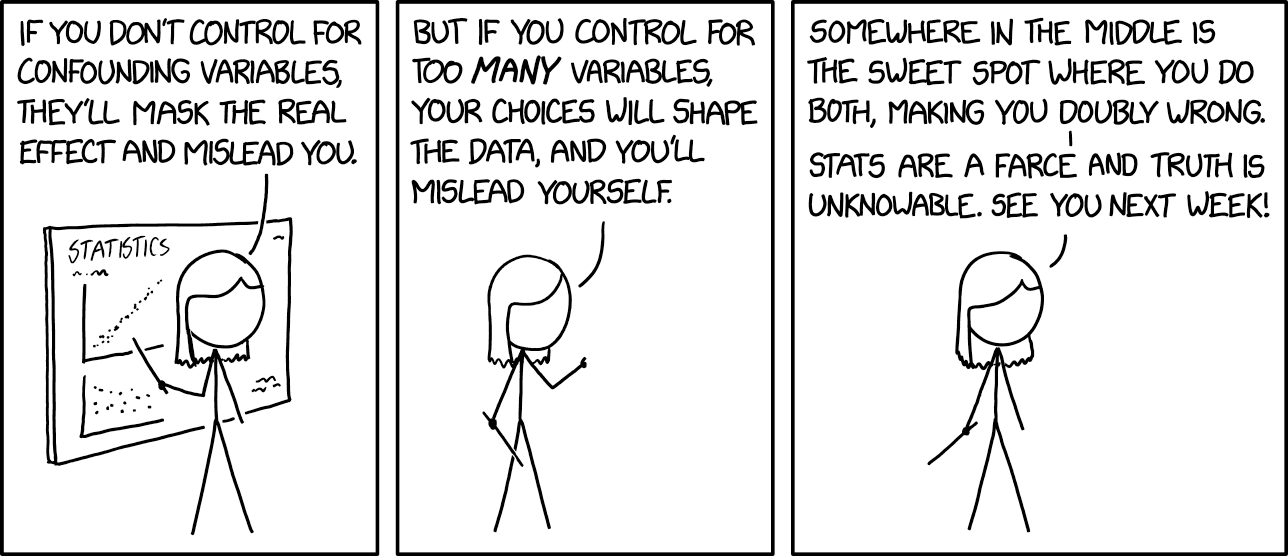
\includegraphics{images/confounding_variables.png}
\end{center}

\setlength{\abovedisplayskip}{-5pt}
\setlength{\abovedisplayshortskip}{-5pt}

{
\hypersetup{linkcolor=}
\setcounter{tocdepth}{2}
\tableofcontents
}
\listoffigures
\listoftables
\hypertarget{prefazione}{%
\chapter*{Prefazione}\label{prefazione}}


\emph{Data Science per psicologi} contiene il materiale delle lezioni dell'insegnamento di \emph{Psicometria B000286} (A.A. 2021/2022) rivolto agli studenti del primo anno del Corso di Laurea in Scienze e Tecniche Psicologiche dell'Università degli Studi di Firenze. \emph{Psicometria} si propone di fornire agli studenti un'introduzione all'analisi dei dati in psicologia. Le conoscenze/competenze che verranno sviluppate in questo insegnamento sono quelle della Data science, ovvero un insieme di conoscenze/competenze che si pongono all'intersezione tra statistica (ovvero, richiedono la capacità di comprendere teoremi statistici) e informatica (ovvero, richiedono la capacità di sapere utilizzare un software).

\hypertarget{la-psicologia-e-la-data-science}{%
\section*{La psicologia e la Data science}\label{la-psicologia-e-la-data-science}}


Sembra sensato spendere due parole su un tema che è importante per gli studenti: quello indicato dal titolo di questo Capitolo. È ovvio che agli studenti di psicologia la statistica non piace. Se piacesse, forse studierebbero Data science e non psicologia; ma non lo fanno. Di conseguenza, gli studenti di psicologia si chiedono: ``perché dobbiamo perdere tanto tempo a studiare queste cose quando in realtà quello che ci interessa è tutt'altro?'' Questa è una bella domanda.

C'è una ragione molto semplice che dovrebbe farci capire perché la Data science è così importante per la psicologia. Infatti, a ben pensarci, la psicologia è una disciplina intrinsecamente statistica, se per statistica intendiamo quella disciplina che studia la variazione delle caratteristiche degli individui nella popolazione. La psicologia studia \emph{gli individui} ed è proprio la variabilità inter- e intra-individuale ciò che vogliamo descrivere e, in certi casi, predire. In questo senso, la psicologia è molto diversa dall'ingegneria, per esempio. Le proprietà di un determinato ponte sotto certe condizioni, ad esempio, sono molto simili a quelle di un altro ponte, sotto le medesime condizioni. Quindi, per un ingegnere la statistica è poco importante: le proprietà dei materiali sono unicamente dipendenti dalla loro composizione e restano costanti. Ma lo stesso non può dirsi degli individui: ogni individuo è unico e cambia nel tempo. E le variazioni tra gli individui, e di un individuo nel tempo, sono l'oggetto di studio proprio della psicologia: è dunque chiaro che i problemi che la psicologia si pone sono molto diversi da quelli affrontati, per esempio, dagli ingegneri. Questa è la ragione per cui abbiamo tanto bisogno della Data science in psicologia: perché la Data science ci consente di descrivere la variazione e il cambiamento. E queste sono appunto le caratteristiche di base dei fenomeni psicologici.

Sono sicuro che, leggendo queste righe, a molti studenti sarà venuta in mente la seguente domanda: perché non chiediamo a qualche esperto di fare il ``lavoro sporco'' (ovvero le analisi statistiche) per noi, mentre noi (gli psicologi) ci occupiamo solo di ciò che ci interessa, ovvero dei problemi psicologici slegati dai dettagli ``tecnici'' della Data science? La risposta a questa domanda è che non è possibile progettare uno studio psicologico sensato senza avere almeno una comprensione rudimentale della Data science. Le tematiche della Data science non possono essere ignorate né dai ricercatori in psicologia né da coloro che svolgono la professione di psicologo al di fuori dell'Università. Infatti, anche i professionisti al di fuori dall'università non possono fare a meno di leggere la letteratura psicologica più recente: il continuo aggiornamento delle conoscenze è infatti richiesto dalla deontologia della professione. Ma per potere fare questo è necessario conoscere un bel po' di Data science! Basta aprire a caso una rivista specialistica di psicologia per rendersi conto di quanto ciò sia vero: gli articoli che riportano i risultati delle ricerche psicologiche sono zeppi di analisi statistiche e di modelli formali. E la comprensione della letteratura psicologica rappresenta un requisito minimo nel bagaglio professionale dello psicologo.

Le considerazioni precedenti cercano di chiarire il seguente punto: la Data science non è qualcosa da studiare a malincuore, in un singolo insegnamento universitario, per poi poterla tranquillamente dimenticare. Nel bene e nel male, gli psicologi usano gli strumenti della Data science in tantissimi ambiti della loro attività professionale: in particolare quando costruiscono, somministrano e interpretano i test psicometrici. È dunque chiaro che possedere delle solide basi di Data science è un tassello imprescindibile del bagaglio professionale dello psicologo. In questo insegnamento verrano trattati i temi base della Data science e verrà adottato un punto di vista bayesiano, che corrisponde all'approccio più recente e sempre più diffuso in psicologia.

\hypertarget{come-studiare}{%
\section*{Come studiare}\label{come-studiare}}


Il giusto metodo di studio per prepararsi all'esame di Psicometria è quello di seguire attivamente le lezioni, assimilare i concetti via via che essi vengono presentati e verificare in autonomia le procedure presentate a lezione. Incoraggio gli studenti a farmi domande per chiarire ciò che non è stato capito appieno. Incoraggio gli studenti a utilizzare i forum attivi su Moodle e, soprattutto, a svolgere gli esercizi proposti su Moodle. I problemi forniti su Moodle rappresentano il livello di difficoltà richiesto per superare l'esame e consentono allo studente di comprendere se le competenze sviluppate fino a quel punto sono sufficienti rispetto alle richieste dell'esame.

La prima fase dello studio, che è sicuramente individuale, è quella in cui è necessario acquisire le conoscenze teoriche relative ai problemi che saranno presentati all'esame. La seconda fase di studio, che può essere facilitata da scambi con altri e da incontri di gruppo, porta ad acquisire la capacità di applicare le conoscenze: è necessario capire come usare un software (\(\textsf{R}\)) per applicare i concetti statistici alla specifica situazione del problema che si vuole risolvere. Le due fasi non sono però separate: il saper fare molto spesso ci aiuta a capire meglio.

\hypertarget{sviluppare-un-metodo-di-studio-efficace}{%
\section*{Sviluppare un metodo di studio efficace}\label{sviluppare-un-metodo-di-studio-efficace}}


Avendo insegnato molte volte in passato un corso introduttivo di analisi dei dati ho notato nel corso degli anni che gli studenti con l'atteggiamento mentale che descriverò qui sotto generalmente ottengono ottimi risultati. Alcuni studenti sviluppano naturalmente questo approccio allo studio, ma altri hanno bisogno di fare uno sforzo per maturarlo. Fornisco qui sotto una breve descrizione del ``metodo di studio'' che, nella mia esperienza, è il più efficace per affrontare le richieste di questo insegnamento.

\begin{itemize}
\tightlist
\item
  Dedicate un tempo sufficiente al materiale di base, apparentemente facile; assicuratevi di averlo capito bene. Cercate le lacune nella vostra comprensione. Leggere presentazioni diverse dello stesso materiale (in libri o articoli diversi) può fornire nuove intuizioni.
\item
  Gli errori che facciamo sono i nostri migliori maestri. Istintivamente cerchiamo di dimenticare subito i nostri errori. Ma il miglior modo di imparare è apprendere dagli errori che commettiamo. In questo senso, una soluzione corretta è meno utile di una soluzione sbagliata. Quando commettiamo un errore questo ci fornisce un'informazione importante: ci fa capire qual è il materiale di studio sul quale dobbiamo ritornare e che dobbiamo capire meglio.
\item
  C'è ovviamente un aspetto ``psicologico'' nello studio. Quando un esercizio o problema ci sembra incomprensibile, la cosa migliore da fare è dire: ``mi arrendo'', ``non ho idea di cosa fare!''. Questo ci rilassa: ci siamo già arresi, quindi non abbiamo niente da perdere, non dobbiamo più preoccuparci. Ma non dobbiamo fermarci qui. Le cose ``migliori'' che faccio (se ci sono) le faccio quando non ho voglia di lavorare. Alle volte, quando c'è qualcosa che non so fare e non ho idea di come affontare, mi dico: ``oggi non ho proprio voglia di fare fatica'', non ho voglia di mettermi nello stato mentale per cui ``in 10 minuti devo risolvere il problema perché dopo devo fare altre cose''. Però ho voglia di \emph{divertirmi} con quel problema e allora mi dedico a qualche aspetto ``marginale'' del problema, che so come affrontare, oppure considero l'aspetto più difficile del problema, quello che non so come risolvere, ma invece di cercare di risolverlo, guardo come altre persone hanno affrontato problemi simili, opppure lo stesso problema in un altro contesto. Non mi pongo l'obiettivo ``risolvi il problema in 10 minuti'', ma invece quello di farmi un'idea ``generale'' del problema, o quello di capire un caso più specifico e più semplice del problema. Senza nessuna pressione. Infatti, in quel momento ho deciso di non lavorare (ovvero, di non fare fatica). Va benissimo se ``parto per la tangente'', ovvero se mi metto a leggere del materiale che sembra avere poco a che fare con il problema centrale (le nostre intuizioni e la nostra curiosità solitamente ci indirizzano sulla strada giusta). Quando faccio così, molto spesso trovo la soluzione del problema che mi ero posto e, paradossalmente, la trovo in un tempo minore di quello che, in precedenza, avevo dedicato a ``lavorare'' al problema. Allora perché non faccio sempre così? C'è ovviamente l'aspetto dei ``10 minuti'' che non è sempre facile da dimenticare. Sotto pressione, possiamo solo agire in maniera automatica, ovvero possiamo solo applicare qualcosa che già sappiamo fare. Ma se dobbiamo imparare qualcosa di nuovo, la pressione è un impedimento.
\item
  È utile farsi da soli delle domande sugli argomenti trattati, senza limitarsi a cercare di risolvere gli esercizi che vengono assegnati. Quando studio qualcosa mi viene in mente: ``se questo è vero, allora deve succedere quest'altra cosa''. Allora verifico se questo è vero, di solito con una simulazione. Se i risultati della simulazione sono quelli che mi aspetto, allora vuol dire che ho capito. Se i risultati sono diversi da quelli che mi aspettavo, allora mi rendo conto di non avere capito e ritorno indietro a studiare con più attenzione la teoria che pensavo di avere capito -- e ovviamente mi rendo conto che c'era un aspetto che avevo frainteso. Questo tipo di verifica è qualcosa che dobbiamo fare da soli, in prima persona: nessun altro può fare questo al posto nostro.
\item
  Non aspettatevi di capire tutto la prima volta che incontrate un argomento nuovo.\footnote{Ricordatevi inoltre che gli individui tendono a sottostimare la propria capacità di apprendere \citep{horn2021underestimating}.} È utile farsi una nota mentalmente delle lacune nella vostra comprensione e tornare su di esse in seguito per carcare di colmarle. L'atteggiamento naturale, quando non capiamo i dettagli di qualcosa, è quello di pensare: ``non importa, ho capito in maniera approssimativa questo punto, non devo preoccuparmi del resto''. Ma in realtà non è vero: se la nostra comprensione è superficiale, quando il problema verrà presentato in una nuova forma, non riusciremo a risolverlo. Per cui i dubbi che ci vengono quando studiamo qualcosa sono il nostro alleato più prezioso: ci dicono esattamente quali sono gli aspetti che dobbiamo approfondire per potere migliorare la nostra preparazione.
\item
  È utile sviluppare una visione d'insieme degli argomenti trattati, capire l'obiettivo generale che si vuole raggiungere e avere chiaro il contributo che i vari pezzi di informazione forniscono al raggiungimento di tale obiettivo. Questa organizzazione mentale del materiale di studio facilita la comprensione. È estremamente utile creare degli schemi di ciò che si sta studiando. Non aspettate che sia io a fornirvi un riepilogo di ciò che dovete imparare: sviluppate da soli tali schemi e tali riassunti.
\item
  Tutti noi dobbiamo imparare l'arte di trovare le informazioni, non solo nel caso di questo insegnamento. Quando vi trovate di fronte a qualcosa che non capite, o ottenete un oscuro messaggio di errore da un software, ricordatevi: ``Google is your friend''!
\end{itemize}

\begin{flushright}
Corrado Caudek\\
Marzo 2022 \end{flushright}

\mainmatter

\hypertarget{part-inferenza-bayesiana}{%
\part{Inferenza bayesiana}\label{part-inferenza-bayesiana}}

\hypertarget{ch:intro-bayes-inference}{%
\chapter{Flusso di lavoro bayesiano}\label{ch:intro-bayes-inference}}

La moderna statistica bayesiana viene per lo più eseguita utilizzando un linguaggio di programmazione probabilistico implementato su computer. Ciò ha cambiato radicalmente il modo in cui venivano eseguite le statistiche bayesiane anche fin pochi decenni fa. La complessità dei modelli che possiamo costruire è aumentata e la barriera delle competenze matematiche e computazionali che sono richieste è diminuita. Inoltre, il processo di modellazione iterativa è diventato, sotto molti aspetti, molto più facile da eseguire. Anche se formulare modelli statistici complessi è diventato più facile che mai, la statistica è un campo pieno di sottigliezze che non scompaiono magicamente utilizzando potenti metodi computazionali. Pertanto, avere una buona preparazione sugli aspetti teorici, specialmente quelli rilevanti nella pratica, è estremamente utile per applicare efficacemente i metodi statistici.

\hypertarget{modellizzazione-bayesiana}{%
\section{Modellizzazione bayesiana}\label{modellizzazione-bayesiana}}

L'analisi bayesiana corrisponde alla costruzione di un modello statistico che si può rappresentare con una quaterna

\begin{equation}
(\mathcal{Y}, p(y \mid \theta), p(\theta), \theta \in \Theta),
\end{equation}

dove \(\mathcal{Y}\) è l'insieme di tutti i possibili risultati ottenuti dall'esperimento casuale e \(p(y \mid \theta)\) è una famiglia di leggi di probabilità, indicizzata dal parametro \(\theta \in \Theta\), che descrive l'incertezza sull'esito dell'esperimento. Secondo l'approccio bayesiano, il parametro incognito \(\theta\) è considerato una variabile casuale che segue la legge di probabilità \(p(\theta)\). L'incertezza su \(\theta\) è la sintesi delle opinioni e delle informazioni che si hanno sul parametro prima di avere osservato il risultato dell'esperimento e prende il nome di \emph{distribuzione a priori}. La costruzione del modello statistico passa attraverso la scelta di una densità \(p(y \mid \theta)\) che rappresenta, in senso probabilistico, il fenomeno d'interesse, e attraverso la scelta di una distribuzione a priori \(p(\theta)\). Le informazioni che si hanno a priori sul parametro di interesse \(\theta\), contenute in \(p(\theta)\), vengono aggiornate attraverso quelle provenienti dal campione osservato \(y = (y_1, \dots, y_n)\) contenute nella funzione \(p(y \mid \theta)\), che, osservata come funzione di \(\theta\) per \(y\), prende il nome di \emph{funzione di verosimiglianza}. L'aggiornamento delle informazioni avviene attraverso la formula di Bayes

\begin{equation}
p(\theta \mid y) = \frac{p(y \mid \theta) p(\theta)}{\int_{\Theta}p(y \mid \theta) p(\theta) \,\operatorname {d}\!\theta} \quad \theta \in \Theta,
 \label{eq:bayes-intro}
\end{equation}

in cui \(p(\theta \mid y)\) prende il nome di \emph{distribuzione a posteriori}.

Il denominatore del Teorema di Bayes \eqref{eq:bayes-intro}, che costituisce la costante di normalizzazione, è la densità marginale dei dati (o verosimiglianza marginale). In ambito bayesiano la distribuzione a posteriori viene utilizzata per calcolare le principali quantità di interesse dell'inferenza, ad esempio la media a posteriori di \(\theta\).

Possiamo descrivere la modellazione bayesiana distinguendo tre passaggi \citep{martin2022bayesian}.

\begin{enumerate}
\def\labelenumi{\arabic{enumi}.}
\tightlist
\item
  Dati alcuni dati e alcune ipotesi su come questi dati potrebbero essere stati generati, progettiamo un modello combinando e trasformando variabili casuali.
\item
  Usiamo il teorema di Bayes per condizionare i nostri modelli ai dati disponibili. Chiamiamo questo processo ``inferenza'' e come risultato otteniamo una distribuzione a posteriori.
\item
  Critichiamo il modello verificando se il modello abbia senso utilizzando criteri diversi, inclusi i dati e la nostra conoscenza del dominio. Poiché generalmente siamo incerti sui modelli, a volte confrontiamo modelli diversi.
\end{enumerate}

Questi tre passaggi vengono eseguiti in modo iterativo e danno luogo a quello che è chiamato ``flusso di lavoro bayesiano'' (\emph{bayesian workflow}).

\hypertarget{notazione}{%
\subsection{Notazione}\label{notazione}}

Per fissare la notazione, nel seguito \(y\) rappresenterà i dati e \(\theta\) rappresenterà i parametri incogniti di un modello statistico. Sia \(y\) che \(\theta\) vengono concepiti come variabili casuali. Con \(x\) vengono invece denotate le quantità note, come ad esempio i predittori del modello lineare. Per rappresentare in un modo conciso i modelli probabilistici viene usata una notazione particolare. Ad esempio, invece di scrivere \(p(\theta) = \mbox{Beta}(1, 1)\) scriviamo \(\theta \sim \mbox{Beta}(1, 1)\). Il simbolo ``\(\sim\)'' viene spesso letto ``è distribuito come''. Possiamo anche pensare che significhi che \(\theta\) costituisce un campione casuale estratto dalla distribuzione Beta(1, 1). Allo stesso modo, ad esempio, la verosimiglianza del modello binomiale può essere scritta come \(y \sim \text{Bin}(n, \theta)\).

\hypertarget{distribuzioni-a-priori}{%
\section{Distribuzioni a priori}\label{distribuzioni-a-priori}}

Quando adottiamo un approccio bayesiano, i parametri della distribuzione di riferimento non venono considerati come delle costanti incognite ma bensì vengono trattati come variabili casuali; di conseguenza, i parametri assumono una particolare distribuzione che nelle statistica bayesiana viene definita ``a priori''. I parametri (o il parametro), che possiamo indicare con \(\theta\), possono assumere delle distribuzioni a priori differenti: a seconda delle informazioni disponibili bisogna selezionare una distribuzione di \(\theta\) in modo tale che venga assegnata una probabilità maggiore a quei valori che si ritengono più plausibili per \(\theta\). Idealmente, le credenze a priori che portano alla specificazione di una distribuzione a priori dovrebbero essere supportate da una qualche motivazione, come ad esempio i risultati di ricerche precedenti.

\hypertarget{tipologie-di-distribuzioni-a-priori}{%
\subsection{Tipologie di distribuzioni a priori}\label{tipologie-di-distribuzioni-a-priori}}

Possiamo distinguere tra diverse distribuzioni a priori in base a quanto fortemente impegnano il ricercatore a ritenere come plausibile un particolare intervallo di valori dei parametri. Il caso più estremo è quello che rivela una totale assenza di conoscenze a priori, il che conduce alle \emph{distribuzioni a priori non informative}, ovvero quelle che assegnano lo stesso livello di credibilità a tutti i valori dei parametri. Le distribuzioni a priori informative, d'altra parte, possono essere \emph{debolmente informative} o \emph{fortemente informative}, a seconda della forza della credenza che esprimono. Il caso più estremo di credenza a priori è quello che riassume il punto di vista del ricercatore nei termini di un \emph{unico valore} del parametro, il che assegna tutta la probabilità (massa o densità) ad di un singolo valore del parametro. Poiché questa non è più una distribuzione di probabilità, sebbene ne soddisfi la definizione, in questo caso si parla di una \emph{distribuzione a priori degenerata}. La figura seguente motra alcuni esempi di distribuzioni a priori per il modello Binomiale:

\begin{itemize}
\tightlist
\item
  distribuzione \emph{non informativa}: \(\theta_c \sim \mbox{Beta}(1,1)\);
\item
  distribuzione \emph{debolmente informativa}: \(\theta_c \sim \mbox{Beta}(5,2)\);
\item
  distribuzione \emph{fortemente informativa}: \(\theta_c \sim \mbox{Beta}(50,20)\);
\item
  \emph{valore puntuale}: \(\theta_c \sim \mbox{Beta}(\alpha, \beta)\) con \(\alpha, \beta \rightarrow \infty\) e \(\frac{\alpha}{\beta} = \frac{5}{2}\).
\end{itemize}

\begin{figure}[h]

{\centering 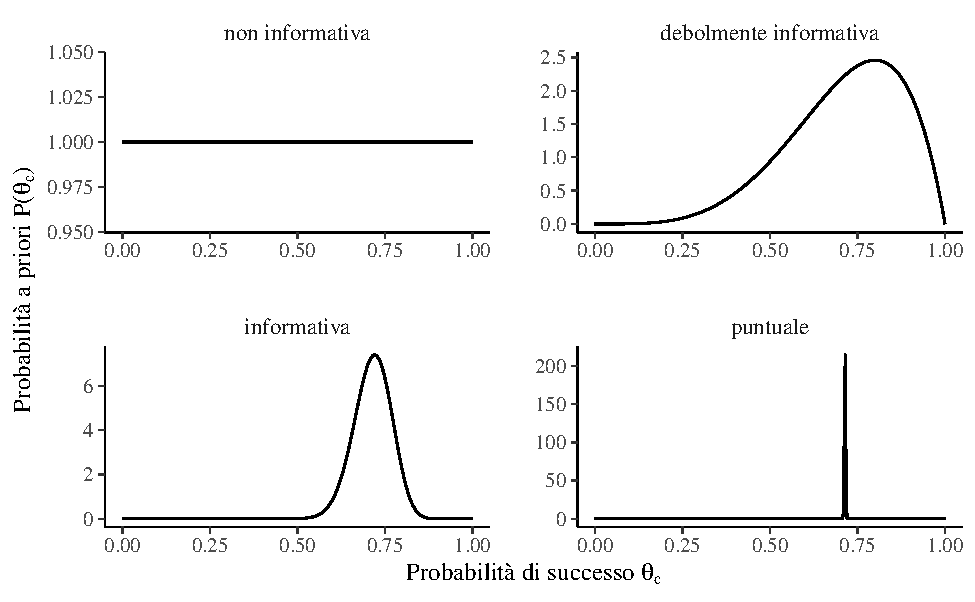
\includegraphics{ds4psy_files/figure-latex/unnamed-chunk-3-1} 

}

\caption{Esempi di distribuzioni a priori per il parametro $\theta_c$ nel Modello Binomiale.}\label{fig:unnamed-chunk-3}
\end{figure}

\hypertarget{selezione-della-distribuzione-a-priori}{%
\subsection{Selezione della distribuzione a priori}\label{selezione-della-distribuzione-a-priori}}

La selezione delle distribuzioni a priori è stata spesso vista come una delle scelte più importanti che un ricercatore fa quando implementa un modello bayesiano in quanto può avere un impatto sostanziale sui risultati finali. La soggettività delle distribuzioni a priori è evidenziata dai critici come un potenziale svantaggio dei metodi bayesiani. A questa critica, \citet{vandeSchoot2021modelling} rispondono dicendo che, al di là della scelta delle distribuzioni a priori, ci sono molti elementi del processo di inferenza statistica che sono soggettivi, ovvero la scelta del modello statistico e le ipotesi sulla distribuzione degli errori. In secondo luogo, \citet{vandeSchoot2021modelling} notano come le distribuzioni a priori svolgono due importanti ruoli statistici: quello della ``regolarizzazione della stima'', ovvero, il processo che porta ad indebolire l'influenza indebita di osservazioni estreme, e quello del miglioramento dell'efficienza della stima, ovvero, la facilitazione dei processi di calcolo numerico di stima della distribuzione a posteriori. L'effetto della distribuzione a priori sulla distribuzione a posteriori verrà discusso in dettaglio nel Capitolo \ref{chapter-balance}.

\hypertarget{un-esempio-concreto}{%
\subsection{Un esempio concreto}\label{un-esempio-concreto}}

Per introdurre la modelizzazione bayesiana useremo qui i dati riportati da \citet{zetschefuture2019} (si veda l'appendice \ref{appendix:future-exp}). Tali dati corrispondono a 23 ``successi'' in 30 prove e possono dunque essere considerati la manifestazione di una variabile casuale Bernoulliana.

Se non abbiamo alcuna informazione a priori su \(\theta\) (ovvero, la probabilità che l'aspettativa dell'umore futuro del partecipante sia distorta negativamente), potremmo pensare di usare una distribuzione a priori uniforme, ovvero una Beta di parametri \(\alpha=1\) e \(\beta=1\). Una tale scelta, tuttavia, è sconsigliata in quanto è più vantaggioso usare una distribuzione debolmente informativa, come ad esempio \(\mbox{Beta}(2, 2)\), che ha come scopo la regolarizzazione, cioè quello di mantenere le inferenze in un intervallo ragionevole. Qui useremo una \(\mbox{Beta}(2, 10)\).

\[
p(\theta) = \frac{\Gamma(12)}{\Gamma(2)\Gamma(10)}\theta^{2-1} (1-\theta)^{10-1}.
\]

\begin{Shaded}
\begin{Highlighting}[]
\NormalTok{bayesrules}\SpecialCharTok{::}\FunctionTok{plot\_beta}\NormalTok{(}\AttributeTok{alpha =} \DecValTok{2}\NormalTok{, }\AttributeTok{beta =} \DecValTok{10}\NormalTok{, }\AttributeTok{mean =} \ConstantTok{TRUE}\NormalTok{, }\AttributeTok{mode =} \ConstantTok{TRUE}\NormalTok{)}
\end{Highlighting}
\end{Shaded}

\begin{center}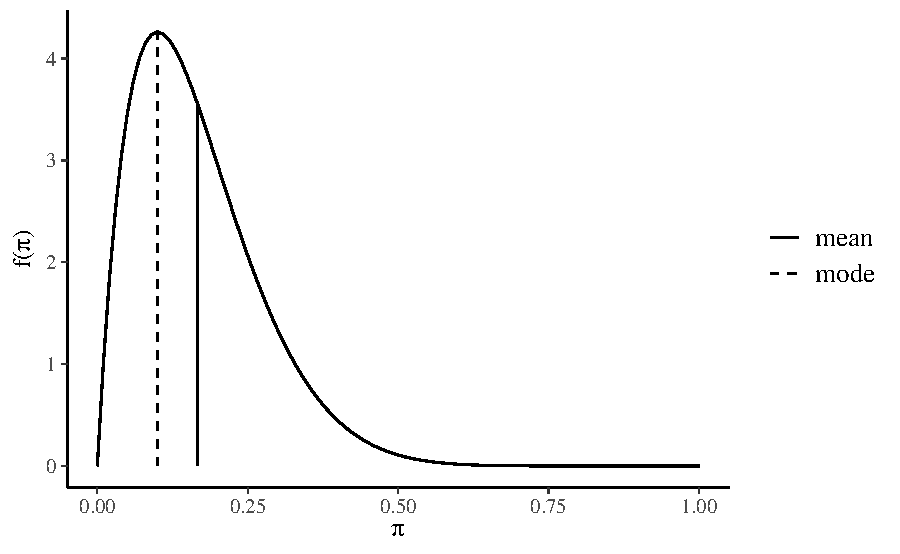
\includegraphics{ds4psy_files/figure-latex/unnamed-chunk-4-1} \end{center}

La \(\mbox{Beta}(2, 10)\) esprime la credenza che \(\theta\) assume valori \(< 0.5\), con il valore più plausibile pari a circa 0.1. Questo è assolutamente implausibile per il caso dell'esempio in discussione: la \(\mbox{Beta}(2, 10)\) verrà usata solo per scopi didattici, ovvero, per esplorare le conseguenze di tale scelta sulla distribuzione a posteriori.

\hypertarget{la-funzione-di-verosimiglianza}{%
\section{La funzione di verosimiglianza}\label{la-funzione-di-verosimiglianza}}

Iniziamo con una definizione.

\begin{definition}
La \emph{funzione di verosimiglianza} \(\mathcal{L}(\theta \mid y) = f(y \mid \theta), \theta \in \Theta,\) è la funzione di massa o di densità di probabilità dei dati \(y\) vista come una funzione del parametro sconosciuto (o dei parametri sconosciuti) \(\theta\).
\end{definition}

Detto in altre parole, le funzioni di verosimiglianza e di (massa o densità di) probabilità sono formalmente identiche, ma è completamente diversa la loro interpretazione. Nel caso della funzione di massa o di densità di probabilità la distribuzione del vettore casuale delle osservazioni campionarie \(y\) dipende dai valori assunti dal parametro (o dai parametri) \(\theta\); nel caso della la funzione di verosimiglianza la credibilità assegnata a ciascun possibile valore \(\theta\) viene determinata avendo acquisita l'informazione campionaria \(y\) che rappresenta l'elemento condizionante. In altri termini, la funzione di verosimiglianza descrive in termini relativi il sostegno empirico che \(\theta \in \Theta\) riceve da \(y\). Infatti, la funzione di verosimiglianza assume forme diverse al variare di \(y\). Possiamo dunque pensare alla funzione di verosimiglianza come alla risposta alla seguente domanda: avendo osservato i dati \(y\), quanto risultano (relativamente) credibili i diversi valori del parametro \(\theta\)? In termini più formali possiamo dire: sulla base dei dati, \(\theta_1 \in \Theta\) risulta più credibile di \(\theta_2 \in \Theta\) quale indice del modello probabilistico generatore dei dati se \(\mathcal{L}(\theta_1) > \mathcal{L}(\theta_1)\).

Notiamo un punto importante: la funzione \(\mathcal{L}(\theta \mid y)\) non è una funzione di densità. Infatti, essa non racchiude un'area unitaria.

\hypertarget{notazione-1}{%
\subsection{Notazione}\label{notazione-1}}

Seguendo una pratica comune, in questa dispensa spesso useremo la notazione \(p(\cdot)\) per rappresentare due quantità differenti, ovvero la funzione di verosimiglianza e la distribuzione a priori. Questo piccolo abuso di notazione riflette il seguente punto di vista: anche se la verosimiglianza non è una funzione di densità di probabilità, noi non vogliamo stressare questo aspetto, ma vogliamo piuttosto pensare alla verosimiglianza e alla distribuzione a priori come a due elementi che sono egualmente necessari per calcolare la distribuzione a posteriori. In altri termini, per così dire, questa notazione assegna lo stesso status epistemologico alle due diverse quantità che si trovano al numeratore della regola di Bayes.

\hypertarget{la-log-verosimiglianza}{%
\subsection{La log-verosimiglianza}\label{la-log-verosimiglianza}}

Dal punto di vista pratico risulta più conveniente utilizzare, al posto della funzione di verosimiglianza, il suo logaritmo naturale, ovvero la funzione di log-verosimiglianza:

\begin{equation}
\ell(\theta) = \log \mathcal{L}(\theta).
\end{equation}

Poiché il logaritmo è una funzione strettamente crescente (usualmente si considera il logaritmo naturale), allora \(\mathcal{L}(\theta)\) e \(\ell(\theta)\) assumono il massimo (o i punti di massimo) in corrispondenza degli stessi valori di \(\theta\) (per un approfondimento, si veda l'Appendice \ref{appendix:max-like}):

\[
\hat{\theta} = \argmax_{\theta \in \Theta} \ell(\theta) = \argmax_{\theta \in \Theta} \mathcal{L}(\theta).
\]

Per le proprietà del logaritmo, si ha

\begin{equation}
\ell(\theta) = \log \left( \prod_{i = 1}^n f(y \mid \theta) \right) = \sum_{i = 1}^n \log f(y \mid \theta).
\end{equation}

Si noti che non è necessario lavorare con i logaritmi, ma è fortemente consigliato. Il motivo è che i valori della verosimiglianza, in cui si moltiplicano valori di probabilità molto piccoli, possono diventare estremamente piccoli -- qualcosa come \(10^{-34}\). In tali circostanze, non è sorprendente che i programmi dei computer mostrino problemi di arrotondamento numerico. Le trasformazioni logaritmiche risolvono questo problema.

\hypertarget{un-esempio-concreto-1}{%
\subsection{Un esempio concreto}\label{un-esempio-concreto-1}}

Se i dati di \citet{zetschefuture2019} possono essere riassunti da una proporzione allora è sensato adottare un modello probabilistico binomiale quale meccanismo generatore dei dati:

\begin{equation}
y  \sim \mbox{Bin}(n, \theta),
\label{eq:binomialmodel}
\end{equation}

laddove \(\theta\) è la probabiltà che una prova Bernoulliana assuma il valore 1 e \(n\) corrisponde al numero di prove Bernoulliane. Questo modello assume che le prove Bernoulliane \(y_i\) che costituiscono il campione \(y\) siano tra loro indipendenti e che ciascuna abbia la stessa probabilità \(\theta \in [0, 1]\) di essere un ``successo'' (valore 1). In altre parole, il modello generatore dei dati avrà una funzione di massa di probabilità

\[
p(y \mid \theta)
\ = \
\mbox{Bin}(y \mid n, \theta).
\]

Nei capitoli precedenti è stato mostrato come, sulla base del modello binomiale, sia possibile assegnare una probabilità a ciascun possibile valore \(y \in \{0, 1, \dots, n\}\) \emph{assumendo noto il valore del parametro} \(\theta\). Ma ora abbiamo il problema inverso, ovvero quello di fare inferenza su \(\theta\) alla luce dei dati campionari \(y\). In altre parole, riteniamo di conoscere il modello probabilistico che ha generato i dati, ma di tale modello non conosciamo i parametri: vogliamo dunque ottenere informazioni su \(\theta\) avendo osservato i dati \(y\).

Per i dati di \citet{zetschefuture2019} la funzione di verosimiglianza corrisponde alla funzione binomiale di parametro \(\theta \in [0, 1]\) sconosciuto. Abbiamo osservato un ``successo'' 23 volte in 30 ``prove'', dunque, \(y = 23\) e \(n = 30\). La funzione di verosimiglianza diventa

\begin{equation}
\mathcal{L}(\theta \mid y) = \frac{(23 + 7)!}{23!7!} \theta^{23} + (1-\theta)^7.
\label{eq:likebino23}
\end{equation}

Per costruire la funzione di verosimiglianza dobbiamo applicare la \eqref{eq:likebino23} tante volte, cambiando ogni volta il valore \(\theta\) ma \emph{tenendo sempre costante il valore dei dati}. Per esempio, se poniamo \(\theta = 0.1\)

\[
\mathcal{L}(\theta \mid y) = \frac{(23 + 7)!}{23!7!} 0.1^{23} + (1-0.1)^7
\]

otteniamo

\begin{Shaded}
\begin{Highlighting}[]
\FunctionTok{dbinom}\NormalTok{(}\DecValTok{23}\NormalTok{, }\DecValTok{30}\NormalTok{, }\FloatTok{0.1}\NormalTok{)}
\CommentTok{\#\textgreater{} [1] 9.737e{-}18}
\end{Highlighting}
\end{Shaded}

Se poniamo \(\theta = 0.2\)

\[
\mathcal{L}(\theta \mid y) = \frac{(23 + 7)!}{23!7!} 0.2^{23} + (1-0.2)^7
\]

otteniamo

\begin{Shaded}
\begin{Highlighting}[]
\FunctionTok{dbinom}\NormalTok{(}\DecValTok{23}\NormalTok{, }\DecValTok{30}\NormalTok{, }\FloatTok{0.2}\NormalTok{)}
\CommentTok{\#\textgreater{} [1] 3.581e{-}11}
\end{Highlighting}
\end{Shaded}

e così via. La figura \ref{fig:likefutexpect} --- costruita utilizzando 100 valori equispaziati \(\theta \in [0, 1]\) --- fornisce una rappresentazione grafica della funzione di verosimiglianza.

\begin{Shaded}
\begin{Highlighting}[]
\NormalTok{n }\OtherTok{\textless{}{-}} \DecValTok{30}
\NormalTok{y }\OtherTok{\textless{}{-}} \DecValTok{23}
\NormalTok{theta }\OtherTok{\textless{}{-}} \FunctionTok{seq}\NormalTok{(}\DecValTok{0}\NormalTok{, }\DecValTok{1}\NormalTok{, }\AttributeTok{length.out =} \DecValTok{100}\NormalTok{)}
\NormalTok{like }\OtherTok{\textless{}{-}} \FunctionTok{choose}\NormalTok{(n, y) }\SpecialCharTok{*}\NormalTok{ theta}\SpecialCharTok{\^{}}\NormalTok{y }\SpecialCharTok{*}\NormalTok{ (}\DecValTok{1} \SpecialCharTok{{-}}\NormalTok{ theta)}\SpecialCharTok{\^{}}\NormalTok{(n }\SpecialCharTok{{-}}\NormalTok{ y)}
\FunctionTok{tibble}\NormalTok{(theta, like) }\SpecialCharTok{\%\textgreater{}\%}
  \FunctionTok{ggplot}\NormalTok{(}\FunctionTok{aes}\NormalTok{(}\AttributeTok{x =}\NormalTok{ theta, }\AttributeTok{y =}\NormalTok{ like)) }\SpecialCharTok{+}
  \FunctionTok{geom\_line}\NormalTok{() }\SpecialCharTok{+}
  \FunctionTok{labs}\NormalTok{(}
    \AttributeTok{y =} \FunctionTok{expression}\NormalTok{(}\FunctionTok{L}\NormalTok{(theta)),}
    \AttributeTok{x =} \FunctionTok{expression}\NormalTok{(}\StringTok{"Valori possibili di"} \SpecialCharTok{\textasciitilde{}}\NormalTok{ theta)}
\NormalTok{  )}
\end{Highlighting}
\end{Shaded}

\begin{figure}[h]

{\centering 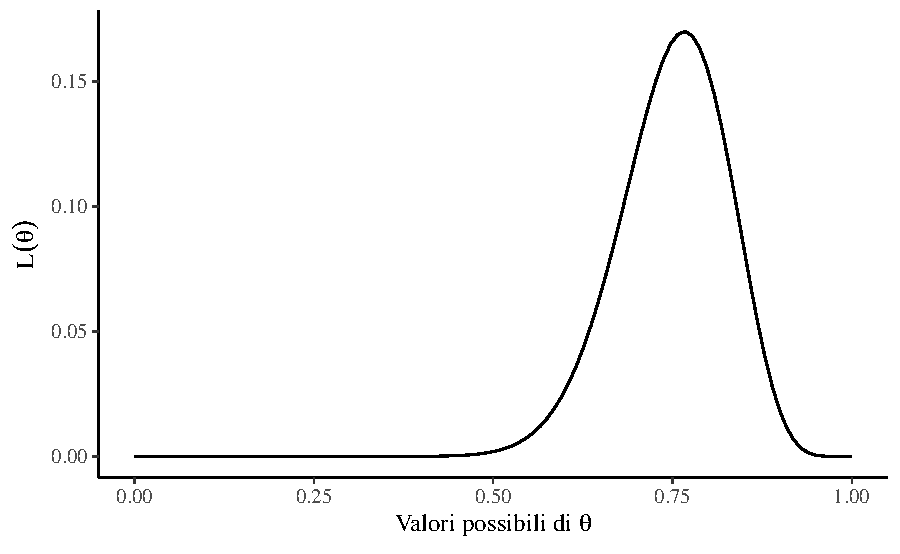
\includegraphics{ds4psy_files/figure-latex/likefutexpect-1} 

}

\caption{Funzione di verosimiglianza nel caso di 23 successi in 30 prove.}\label{fig:likefutexpect}
\end{figure}

Come possiamo interpretare la curva che abbiamo ottenuto? Per alcuni valori \(\theta\) la funzione di verosimiglianza assume valori piccoli; per altri valori \(\theta\) la funzione di verosimiglianza assume valori più grandi. Questi ultimi sono i valori di \(\theta\) più credibili e il valore 23/30 (la moda della funzione di verosimiglianza) è il valore più credibile di tutti.

\hypertarget{sec:const-normaliz-bino23}{%
\section{La verosimiglianza marginale}\label{sec:const-normaliz-bino23}}

Per il calcolo di \(p(\theta \mid y)\) è necessario dividere il prodotto tra la distribuzione a priori e la verosimiglianza per una costante di normalizzazione. Tale costante di normalizzazione, detta \emph{verosimiglianza marginale}, ha lo scopo di fare in modo che \(p(\theta \mid y)\) abbia area unitaria.

Si noti che, nel caso di variabili continue, la verosimiglianza marginale è espressa nei termini di un integrale. Tranne in pochi casi particolari, tale integrale non ha una soluzione analitica. Per questa ragione, l'inferenza bayesiana procede calcolando una approssimazione della distribuzione a posteriori mediante metodi numerici.

\hypertarget{un-esempio-concreto-2}{%
\subsection{Un esempio concreto}\label{un-esempio-concreto-2}}

Consideriamo nuovamente i dati di \citet{zetschefuture2019}. Supponiamo che nel numeratore bayesiano la verosimiglianza sia moltiplicata per una distribuzione uniforme, ovvero \(\mbox{Beta}(1, 1)\). In tali circostanze, il prodotto si riduce alla funzione di verosimiglianza. Per i dati di \citet{zetschefuture2019}, dunque, la costante di normalizzazione si ottiene marginalizzando la funzione di verosimiglianza \(p(y = 23, n = 30 \mid \theta)\) sopra \(\theta\), ovvero risolvendo l'integrale:

\begin{equation}
p(y = 23, n = 30) = \int_0^1 \binom{30}{23} \theta^{23} (1-\theta)^{7} \,\operatorname {d}\!\theta.
\label{eq:intlikebino23}
\end{equation}

Una soluzione numerica si trova facilmente usando \(\R\):

\begin{Shaded}
\begin{Highlighting}[]
\NormalTok{like\_bin }\OtherTok{\textless{}{-}} \ControlFlowTok{function}\NormalTok{(theta) \{}
  \FunctionTok{choose}\NormalTok{(}\DecValTok{30}\NormalTok{, }\DecValTok{23}\NormalTok{) }\SpecialCharTok{*}\NormalTok{ theta}\SpecialCharTok{\^{}}\DecValTok{23} \SpecialCharTok{*}\NormalTok{ (}\DecValTok{1} \SpecialCharTok{{-}}\NormalTok{ theta)}\SpecialCharTok{\^{}}\DecValTok{7}
\NormalTok{\}}
\FunctionTok{integrate}\NormalTok{(like\_bin, }\AttributeTok{lower =} \DecValTok{0}\NormalTok{, }\AttributeTok{upper =} \DecValTok{1}\NormalTok{)}\SpecialCharTok{$}\NormalTok{value}
\CommentTok{\#\textgreater{} [1] 0.03226}
\end{Highlighting}
\end{Shaded}

La derivazione analitica è fornita nell'Appendice \ref{appendix:const-norm-bino23}.

\hypertarget{distribuzione-a-posteriori}{%
\section{Distribuzione a posteriori}\label{distribuzione-a-posteriori}}

La distribuzione a postreriori si trova applicando il teorema di Bayes:

\[
\text{probabilità a posteriori} = \frac{\text{probabilità a priori} \cdot \text{verosimiglianza}}{\text{costante di normalizzazione}}
\]

Una volta trovata la distribuzione a posteriori, possiamo usarla per derivare altre quantità di interesse. Questo viene generalmente ottenuto calcolando il valore atteso:

\[
J = \int f(\theta) p(\theta \mid y) \,\operatorname {d}\!y
\]

Se \(f(\cdot)\) è la funzione identità, ad esempio, \(J\) risulta essere la media di \(\theta\):

\[
\bar{\theta} = \int_{\Theta} \theta p(\theta \mid y) \,\operatorname {d}\!\theta .
\]

Ripeto qui quanto detto sopra: le quantità di interesse della statistica bayesiana(costante di normalizzazione, valore atteso della distribuzione a posteriori, ecc.) contengono integrali che risultano, nella maggior parte dei casi, impossibili da risolvere analiticamente. Per questo motivo, si ricorre a metodi di stima numerici, in particolare a quei metodi Monte Carlo basati sulle proprietà delle catene di Markov (MCMC). Questo argomento verrà discusso nel Capitolo \ref{ch:metropolis}.

\hypertarget{distribuzione-predittiva-a-priori}{%
\section{Distribuzione predittiva a priori}\label{distribuzione-predittiva-a-priori}}

La distribuzione a posteriori è l'oggetto centrale nella statistica bayesiana, ma non è l'unico. Oltre a fare inferenze sui valori dei parametri, potremmo voler fare inferenze sui dati. Questo può essere fatto calcolando la \emph{distribuzione predittiva a priori}:

\begin{equation}
p(y^*) = \int_\Theta p(y^* \mid \theta) p(\theta) \,\operatorname {d}\!\theta .
\label{eq:prior-pred-distr}
\end{equation}

La \eqref{eq:prior-pred-distr} descrive la distribuzione prevista dei dati in base al modello (che include la distribuzione a priori e la verosimiglianza), ovvero descrive i dati \(y^*\) che ci aspettiamo di osservare, dato il modello, prima di avere osservato i dati del campione.

È possibile utilizzare campioni dalla distribuzione predittiva a priori per valutare e calibrare i modelli utilizzando le nostre conoscenze dominio-specifiche. Ad esempio, ci possiamo chiedere: ``È sensato che un modello dell'altezza umana preveda che un essere umano sia alto -1.5 metri?''. Già prima di misurare una singola persona, possiamo renderci conto dell'assurdità di questa domanda. Se la distribuzione prevista dei dati consente domande di questo tipo (ovvero, prevede di osservare dati che risultano insensati alla luce delle nostre conoscenze dominio-specifiche), è chiaro che il modello deve essere riformulato.

\hypertarget{distribuzione-predittiva-a-posteriori}{%
\section{Distribuzione predittiva a posteriori}\label{distribuzione-predittiva-a-posteriori}}

Un'altra quantità utile da calcolare è la distribuzione predittiva a posteriori:

\begin{equation}
p(\tilde{y} \mid y) = \int_\Theta p(\tilde{y} \mid \theta) p(\theta \mid y) \,\operatorname {d}\!\theta .
\label{eq:post-pred-distr}
\end{equation}

Questa è la distribuzione dei dati attesi futuri \(\tilde{y}\) alla luce della distribuzione a posteriori \(p(\theta \mid y)\), che a sua volta è una conseguenza del modello adottato (distribuzione a priori e verosimiglianza) e dei dati osservati. In altre parole, questi sono i dati che il modello si aspetta dopo aver osservato i dati de campione. Dalla \eqref{eq:post-pred-distr} possiamo vedere che le previsioni sui dati attesi futuri sono calcolate integrando (o marginalizzando) sulla distribuzione a posteriori dei parametri. Di conseguenza, le previsioni calcolate in questo modo incorporano l'incertezza relativa alla stima dei parametri del modello.

\hypertarget{commenti-e-considerazioni-finali}{%
\section*{Commenti e considerazioni finali}\label{commenti-e-considerazioni-finali}}


Questo Capitolo ha brevemente passato in rassegna i concetti di base dell'inferenza statistica bayesiana. In base all'approccio bayesiano, invece di dire che il parametro di interesse di un modello statistico ha un valore vero ma sconosciuto, diciamo che, prima di eseguire l'esperimento, è possibile assegnare una distribuzione di probabilità, che chiamano stato di credenza, a quello che è il vero valore del parametro. Questa distribuzione a priori può essere nota (per esempio, sappiamo che la distribuzione dei punteggi del QI è normale con media 100 e deviazione standard 15) o può essere del tutto arbitraria. L'inferenza bayesiana procede poi nel modo seguente: si raccolgono alcuni dati e si calcola la probabilità dei possibili valori del parametro alla luce dei dati osservati e delle credenze a priori. Questa nuova distribuzione di probabilità è chiamata ``distribuzione a posteriori'' e riassume l'incertezza dell'inferenza.

\hypertarget{stan-beta-binom}{%
\chapter{Il modello beta-binomiale in linguaggio Stan}\label{stan-beta-binom}}

In questo Capitolo introdurremo un linguaggio di programmazione probabilistica chiamato Stan. \href{http://mc-stan.org/}{Stan} è un linguaggio di programmazione probabilistica usato per l'inferenza bayesiana \citep{carpenter2017stan}. Prende il nome da uno dei creatori del metodo Monte Carlo, Stanislaw Ulam \citep{Eckhardt1987stan}. Stan consente di generare campioni da distribuzioni di probabilità basati sulla costruzione di una catena di Markov avente come distribuzione di equilibrio (o stazionaria) la distribuzione desiderata. Un'introduzione al linguaggio Stan è fornita nell'Appendice \ref{appendix:intro-stan}. In questo Capitolo useremo Stan per fare inferenza su una proporzione.

\hypertarget{il-presidente-trump-e-lidrossiclorochina}{%
\section{Il presidente Trump e l'idrossiclorochina}\label{il-presidente-trump-e-lidrossiclorochina}}

Per fare un esempio concreto, consideriamo un set di dati reali. Cito dal \emph{Washington Post} del 7 aprile 2020: \emph{``One of the most bizarre and disturbing aspects of President Trump's nightly press briefings on the coronavirus pandemic is when he turns into a drug salesman. Like a cable TV pitchman hawking `male enhancement' pills, Trump regularly extols the virtues of taking hydroxychloroquine, a drug used to treat malaria and lupus, as a potential `game changer' that just might cure Covid-19.''} Tralasciamo qui il fatto che il Donald Trump non sia un esperto in questo campo. Esaminiamo invece le evidenze iniziali a supporto dell'ipotesi che l'idrossiclorochina possa essere utile per la cura del Covid-19, ovvero le evidenze che erano disponibili nel momento in cui il Donald Trump ha fatto le affermazioni riportate sopra (in seguito, quest'idea è stata screditata). Tali evidenze sono state fornite da uno studio di \citet{Gautret_2020}. Il disegno sperimentale di \citet{Gautret_2020} comprende, tra le altre cose, il confronto tra una condizione sperimentale e una condizione di controllo. Il confronto importante è tra la proporzione di paziente positivi al virus SARS-CoV-2 nel gruppo sperimentale (a cui è stata somministrata l'idrossiclorochina; 6 su 14) e la proporzione di paziente positivi nel gruppo di controllo (a cui non è stata somministrata l'idrossiclorochina; ovvero 14 su 16). Obiettivo di questo Capitolo è mostrare come si possa fare inferenza sui dati di \citet{Gautret_2020} usando il linguaggio Stan. Per semplicità, iniziamo considerando solo il gruppo di controllo.

\hypertarget{una-proporzione}{%
\section{Una proporzione}\label{una-proporzione}}

Sulla base di ciò che è stato detto nel Capitolo \ref{chapter-distr-coniugate}, sappiamo che, quando i dati sono rappresentati da una proporzione \(\theta\), e quando utilizziamo una distribuzione a priori Beta per \(\theta\), la distribuzione a posteriori di \(\theta\) è specificata dallo schema beta-binomiale. Se scegliamo, ad esempio, una \(\mbox{Beta}(2, 2)\) quale distribuzione a priori per \(\theta\), il modello diventa:

\begin{align}
y &\sim \mbox{Bin}(n, \theta) \notag\\
\theta &\sim \mbox{Beta}(2, 2),
\label{eq:beta-binom-trump}
\end{align}

dove la prima riga definisce la funzione di verosimiglianza e la seconda riga definisce la distribuzione a priori. Vediamo ora come specificare tale modello beta-binomiale in linguaggio Stan.

\hypertarget{cmdstanr-gautret}{%
\section{\texorpdfstring{Interfaccia \texttt{cmdstanr}}{Interfaccia cmdstanr}}\label{cmdstanr-gautret}}

Nella seguente discussione useremo l'interfaccia \texttt{cmdstanr} di CmdStan.\footnote{I modelli discussi in questo capitolo sono discussi da \citet{gelman1995bayesian} mentre il codice è stato ricavato dalla seguente \href{http://avehtari.github.io/BDA_R_demos/demos_rstan/rstan_demo.html}{pagina web}.}. Carichiamo i pacchetti necessari:

\begin{Shaded}
\begin{Highlighting}[]
\FunctionTok{library}\NormalTok{(}\StringTok{"cmdstanr"}\NormalTok{)}
\FunctionTok{library}\NormalTok{(}\StringTok{"posterior"}\NormalTok{)}
\FunctionTok{rstan\_options}\NormalTok{(}\AttributeTok{auto\_write =} \ConstantTok{TRUE}\NormalTok{) }\CommentTok{\# avoid recompilation of models}
\CommentTok{\# parallelize across all CPUs}
\FunctionTok{options}\NormalTok{(}\AttributeTok{mc.cores =}\NormalTok{ parallel}\SpecialCharTok{::}\FunctionTok{detectCores}\NormalTok{()) }
\CommentTok{\# improve execution time}
\FunctionTok{Sys.setenv}\NormalTok{(}\AttributeTok{LOCAL\_CPPFLAGS =} \StringTok{\textquotesingle{}{-}march=native\textquotesingle{}}\NormalTok{) }
\NormalTok{SEED }\OtherTok{\textless{}{-}} \DecValTok{374237} \CommentTok{\# set random seed for reproducibility}
\end{Highlighting}
\end{Shaded}

Per svolgere l'analisi mediante \texttt{cmdstanr} è necessario prima specificare la struttura del modello bayesiano nella notazione Stan e, poi, eseguire il campionamento dalla distribuzione a posteriori. Esaminiamo questi due passaggi per il caso dell'esempio presente.

\hypertarget{fase-1}{%
\subsection{Fase 1}\label{fase-1}}

Nella prima fase dell'analisi dobbiamo definire i dati, i parametri e il modello. I \emph{dati} devono essere contenuti in un oggetto di classe \texttt{list}. Per l'esempio presente abbiamo:

\begin{Shaded}
\begin{Highlighting}[]
\NormalTok{data1\_list }\OtherTok{\textless{}{-}} \FunctionTok{list}\NormalTok{(}
  \AttributeTok{N =} \DecValTok{16}\NormalTok{,}
  \AttributeTok{y =} \FunctionTok{c}\NormalTok{(}\FunctionTok{rep}\NormalTok{(}\DecValTok{1}\NormalTok{, }\DecValTok{14}\NormalTok{), }\FunctionTok{rep}\NormalTok{(}\DecValTok{0}\NormalTok{, }\DecValTok{2}\NormalTok{))}
\NormalTok{)}
\end{Highlighting}
\end{Shaded}

Il \emph{modello} è \(\Bin(n, \theta)\) e, in linguaggio Stan, può essere specificato come

\begin{Shaded}
\begin{Highlighting}[]
\NormalTok{y }\SpecialCharTok{\textasciitilde{}} \FunctionTok{bernoulli}\NormalTok{(theta);}
\end{Highlighting}
\end{Shaded}

Il modello dipende dal \emph{parametro} \texttt{theta}. In Stan, dobbiamo specificare che \texttt{theta} può essere un qualsiasi numero reale compreso tra 0 e 1. Inoltre, dobbiamo specificare la distribuzione a priori di \(\theta\). Per questo parametro abbiamo scelto una \(\mbox{Beta}(2, 2)\) e, in linguaggio Stan, scriviamo

\begin{Shaded}
\begin{Highlighting}[]
\NormalTok{theta }\SpecialCharTok{\textasciitilde{}} \FunctionTok{beta}\NormalTok{(}\DecValTok{2}\NormalTok{, }\DecValTok{2}\NormalTok{);}
\end{Highlighting}
\end{Shaded}

Memorizziamo ora il modello beta-binomiale specificato in linguaggio Stan come stringa di caratteri nel file \texttt{oneprop.stan}:

\begin{Shaded}
\begin{Highlighting}[]
\NormalTok{modelString }\OtherTok{=} \StringTok{"}
\StringTok{data \{}
\StringTok{  int\textless{}lower=0\textgreater{} N;}
\StringTok{  int\textless{}lower=0, upper=1\textgreater{} y[N];}
\StringTok{\}}
\StringTok{parameters \{}
\StringTok{  real\textless{}lower=0, upper=1\textgreater{} theta;}
\StringTok{\}}
\StringTok{model \{}
\StringTok{  theta \textasciitilde{} beta(2, 2);}
\StringTok{  y \textasciitilde{} bernoulli(theta);}
\StringTok{\}}
\StringTok{"}
\FunctionTok{writeLines}\NormalTok{(modelString, }\AttributeTok{con =} \StringTok{"code/oneprop.stan"}\NormalTok{)}
\end{Highlighting}
\end{Shaded}

\hypertarget{fase-2}{%
\subsection{Fase 2}\label{fase-2}}

Per utilizzare il modello che abbiamo specificato, leggiamo l'indirizzo del file che contiene il codice Stan:

\begin{Shaded}
\begin{Highlighting}[]
\NormalTok{file }\OtherTok{\textless{}{-}} \FunctionTok{file.path}\NormalTok{(}\StringTok{"code"}\NormalTok{, }\StringTok{"oneprop.stan"}\NormalTok{)}
\end{Highlighting}
\end{Shaded}

Compiliamo il codice

\begin{Shaded}
\begin{Highlighting}[]
\NormalTok{mod }\OtherTok{\textless{}{-}} \FunctionTok{cmdstan\_model}\NormalTok{(file)}
\end{Highlighting}
\end{Shaded}

ed eseguiamo il campionamento MCMC con la chiamata

\begin{Shaded}
\begin{Highlighting}[]
\NormalTok{fit1 }\OtherTok{\textless{}{-}}\NormalTok{ mod}\SpecialCharTok{$}\FunctionTok{sample}\NormalTok{(}
  \AttributeTok{data =}\NormalTok{ data1\_list,}
  \AttributeTok{iter\_sampling =}\NormalTok{ 4000L,}
  \AttributeTok{iter\_warmup =}\NormalTok{ 2000L,}
  \AttributeTok{seed =} \DecValTok{84735}\NormalTok{,}
  \AttributeTok{chains =}\NormalTok{ 4L,}
  \AttributeTok{parallel\_chains =}\NormalTok{ 4L,}
  \AttributeTok{refresh =} \DecValTok{0}\NormalTok{,}
  \AttributeTok{thin =} \DecValTok{1}
\NormalTok{)}
\end{Highlighting}
\end{Shaded}

Avendo assunto una distribuzione a priori per il parametro \(\theta\), l'algoritmo procede in maniera ciclica, correggendo la distribuzione a priori di \(\theta\) condizionandola ai valori già generati. Dopo un certo numero di cicli, necessari per portare l'algoritmo a convergenza, i valori estratti possono essere assunti come campionati dalla distribuzione a posteriori di \(\theta\).

Si noti che \texttt{\$sample()} richiede due tipi di informazioni. Innanzitutto, dobbiamo specificare le informazioni sul modello in base a:

\begin{itemize}
\tightlist
\item
  \texttt{mod} = la stringa di caratteri che definisce il modello (qui \texttt{oneprop.stan}),
\item
  \texttt{data} = i dati in formato lista (\texttt{data1\_list}).
\end{itemize}

Dobbiamo inoltre specificare le informazioni sul campionamento MCMC utilizzando tre argomenti aggiuntivi:

\begin{itemize}
\tightlist
\item
  L'argomento \texttt{chains} specifica quante catene di Markov parallele eseguire. Eseguiamo qui quattro catene, quindi otteniamo quattro campioni distinti di valori \(\pi\).
\item
  L'argomento \texttt{iter} specifica il numero desiderato di iterazioni o la lunghezza di ciascuna catena di Markov. Per impostazione predefinita, la prima metà di queste iterazioni è costituita da campioni ``burn-in'' o ``warm-up'' che verranno ignorati. La seconda metà è conservata e costituisce un campione della distribuzione a posteriori.
\item
  L'argomento \texttt{seed} per impostare il numero casuale che genera il seme per una simulazione \texttt{cmdstanr}.
\end{itemize}

\hypertarget{burn-in}{%
\subsection{Burn-in}\label{burn-in}}

Al crescere del numero di passi della catena, la distribuzione di target viene sempre meglio approssimata. All'inizio del campionamento, però, la distribuzione può essere significativamente lontana da quella stazionaria, e ci vuole un certo tempo prima di raggiungere la distribuzione stazionaria di equilibrio, detto, appunto, periodo di \emph{burn-in}. I campioni provenienti da tale parte iniziale della catena vanno tipicamente scartati perché possono non rappresentare accuratamente la distribuzione a posteriori

\hypertarget{inferenza}{%
\subsection{Inferenza}\label{inferenza}}

Un sommario della distribuzione a posteriori si ottiene con:

\begin{Shaded}
\begin{Highlighting}[]
\NormalTok{fit1}\SpecialCharTok{$}\FunctionTok{summary}\NormalTok{(}\FunctionTok{c}\NormalTok{(}\StringTok{"theta"}\NormalTok{))}
\CommentTok{\#\textgreater{} \# A tibble: 1 x 10}
\CommentTok{\#\textgreater{}   variable  mean median     sd    mad    q5   q95  rhat}
\CommentTok{\#\textgreater{}   \textless{}chr\textgreater{}    \textless{}dbl\textgreater{}  \textless{}dbl\textgreater{}  \textless{}dbl\textgreater{}  \textless{}dbl\textgreater{} \textless{}dbl\textgreater{} \textless{}dbl\textgreater{} \textless{}dbl\textgreater{}}
\CommentTok{\#\textgreater{} 1 theta    0.798  0.808 0.0876 0.0872 0.638 0.924  1.00}
\CommentTok{\#\textgreater{} \# ... with 2 more variables: ess\_bulk \textless{}dbl\textgreater{},}
\CommentTok{\#\textgreater{} \#   ess\_tail \textless{}dbl\textgreater{}}
\end{Highlighting}
\end{Shaded}

Creiamo un oggetto di classe \texttt{stanfit}

\begin{Shaded}
\begin{Highlighting}[]
\NormalTok{stanfit1 }\OtherTok{\textless{}{-}}\NormalTok{ rstan}\SpecialCharTok{::}\FunctionTok{read\_stan\_csv}\NormalTok{(fit1}\SpecialCharTok{$}\FunctionTok{output\_files}\NormalTok{())}
\end{Highlighting}
\end{Shaded}

di dimensioni

\begin{Shaded}
\begin{Highlighting}[]
\FunctionTok{dim}\NormalTok{(}\FunctionTok{as.matrix}\NormalTok{(stanfit1, }\AttributeTok{pars =} \StringTok{"theta"}\NormalTok{))}
\CommentTok{\#\textgreater{} [1] 16000     1}
\end{Highlighting}
\end{Shaded}

I primi 10 valori sono presentati qui di seguito

\begin{Shaded}
\begin{Highlighting}[]
\FunctionTok{as.matrix}\NormalTok{(stanfit1, }\AttributeTok{pars =} \StringTok{"theta"}\NormalTok{) }\SpecialCharTok{\%\textgreater{}\%} 
  \FunctionTok{head}\NormalTok{(}\DecValTok{10}\NormalTok{)}
\CommentTok{\#\textgreater{}           parameters}
\CommentTok{\#\textgreater{} iterations  theta}
\CommentTok{\#\textgreater{}       [1,] 0.8521}
\CommentTok{\#\textgreater{}       [2,] 0.7845}
\CommentTok{\#\textgreater{}       [3,] 0.7845}
\CommentTok{\#\textgreater{}       [4,] 0.7551}
\CommentTok{\#\textgreater{}       [5,] 0.7256}
\CommentTok{\#\textgreater{}       [6,] 0.7744}
\CommentTok{\#\textgreater{}       [7,] 0.7744}
\CommentTok{\#\textgreater{}       [8,] 0.8062}
\CommentTok{\#\textgreater{}       [9,] 0.8266}
\CommentTok{\#\textgreater{}      [10,] 0.8499}
\end{Highlighting}
\end{Shaded}

La matrice precedente include i valori assunti dalla catena di Markov, ovvero un insieme di valori plausibili \(\theta\) estratti dalla distribuzione a posteriori. Un tracciato della catena di Markov illustra questa esplorazione rappresentando il valore \(\theta\) sulle ordinate e l'indice progressivo di in ogni iterazione sull'ascissa. Usiamo la funzione \texttt{mcmc\_trace()} del pacchetto \texttt{bayesplot} (Gabry et al.~2019) per costruire il grafico che include tutte e quattro le catene di Markov:

\begin{Shaded}
\begin{Highlighting}[]
\NormalTok{stanfit1 }\SpecialCharTok{\%\textgreater{}\%} 
  \FunctionTok{mcmc\_trace}\NormalTok{(}\AttributeTok{pars =} \FunctionTok{c}\NormalTok{(}\StringTok{"theta"}\NormalTok{), }\AttributeTok{size =} \FloatTok{0.1}\NormalTok{)}
\end{Highlighting}
\end{Shaded}

\begin{figure}[h]

{\centering 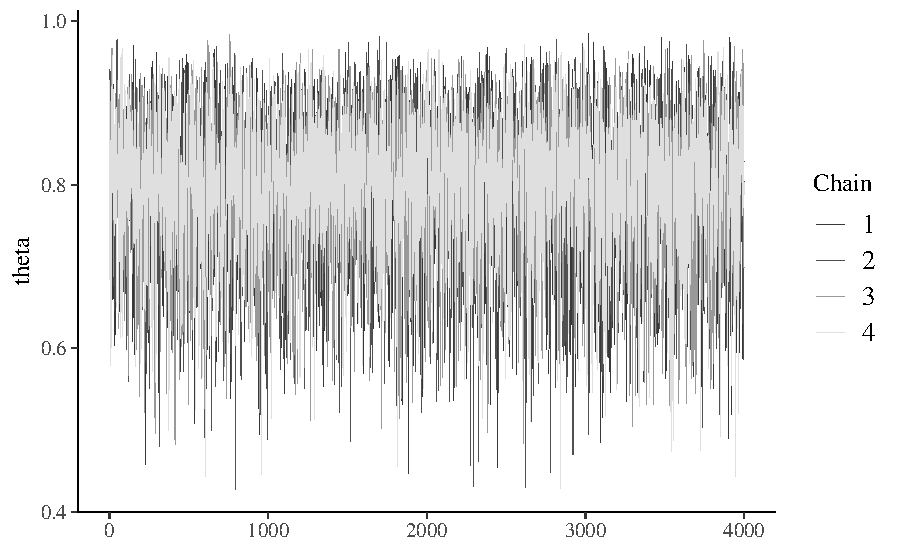
\includegraphics{ds4psy_files/figure-latex/trace-plot-gautret-1} 

}

\caption{Trace-plot per il parametro $\theta$ nel modello Beta-Binomiale.}\label{fig:trace-plot-gautret}
\end{figure}

La figura \ref{fig:trace-plot-gautret} mostra che le catene esplorano uno spazio compreso approssimativamenre tra 0.7 e 0.9; tale figura descrive il comportamento \emph{longitudinale} delle catene di Markov.

Possiamo anche esaminare la distribuzione degli stati della catena di Markov, ovvero, dei valori che queste catene visitano lungo il loro percorso, ignorando l'ordine di queste visite. L'istogramma della figura \ref{fig:hist-post-gautret} fornisce una rappresentazione grafica di questa distribuzione per i 16000 valori complessivi delle quattro catene, ovvero per 4000 valori provienienti da ciascuna catena.

\begin{Shaded}
\begin{Highlighting}[]
\FunctionTok{mcmc\_hist}\NormalTok{(stanfit1, }\AttributeTok{pars =} \StringTok{"theta"}\NormalTok{) }\SpecialCharTok{+} 
  \FunctionTok{yaxis\_text}\NormalTok{(}\ConstantTok{TRUE}\NormalTok{) }\SpecialCharTok{+} 
  \FunctionTok{ylab}\NormalTok{(}\StringTok{"count"}\NormalTok{)}
\end{Highlighting}
\end{Shaded}

\begin{figure}[h]

{\centering 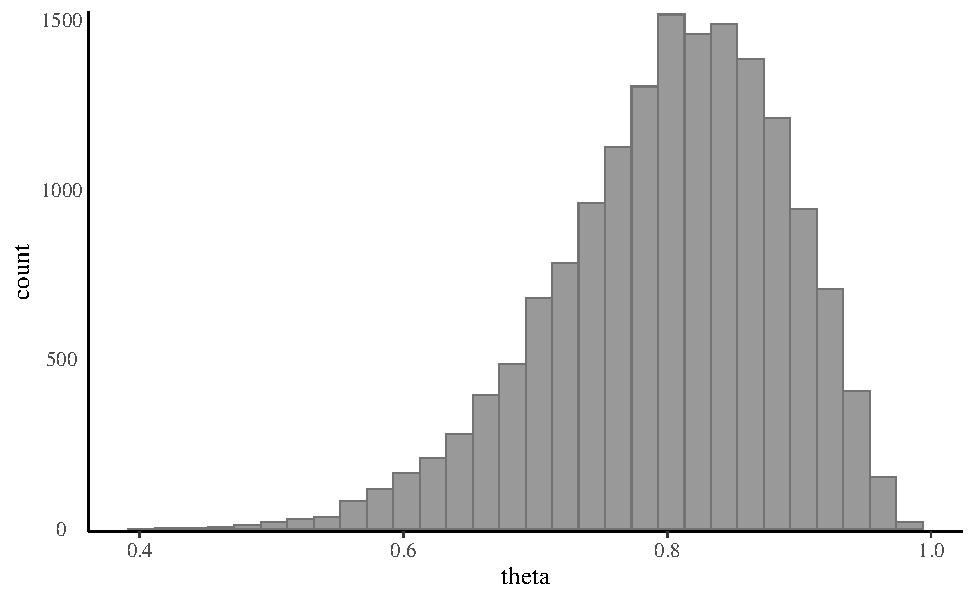
\includegraphics{ds4psy_files/figure-latex/hist-post-gautret-1} 

}

\caption{Istogramma che illustra l'approssimazione della distribuzione a posteriori per il parametro $\theta$ nel modello Beta-Binomiale.}\label{fig:hist-post-gautret}
\end{figure}

Nel modello Beta-Binomiale in cui la verosimiglianza è binomiale con 14 successi su 16 prove e in cui assumiamo una distribuzione a priori di tipo \(\mbox{Beta}(2, 2)\) sul parametro \(\theta\), la distribuzione a posteriori è ancora una distribuzione Beta di parametri \(\alpha\) = 2 + 14 e \(\beta\) = 2 + 16 - 14. La figura \ref{fig:hist-post-gautret-plus-correct} riporta un kernel density plot per i valori delle quattro catene di Markov con sovrapposta in nero la densità \(\mbox{Beta}(16, 4)\). Il punto importante è che la distribuzione dei valori delle catene di Markov produce un'eccellente approssimazione alla distribuzione bersaglio.\footnote{Nel caso presente, il risultato è poco utile dato che è disponibile una soluzione analitica. Tuttavia, questo esercizio mette in evidenza il fatto cruciale che, nei casi in cui possiamo verificarne la soluzione, il campionamento Monte Carlo a catena di Markov è in grado di trovare la risposta corretta. Di conseguenza, possiamo anche essere sicuri che fornirà un'approssimazione alla distribuzione a posteriori anche in quei casi in cui una soluzione analitica non è disponibile.}

\begin{Shaded}
\begin{Highlighting}[]
\FunctionTok{mcmc\_dens}\NormalTok{(stanfit1, }\AttributeTok{pars =} \StringTok{"theta"}\NormalTok{) }\SpecialCharTok{+} 
  \FunctionTok{yaxis\_text}\NormalTok{(}\ConstantTok{TRUE}\NormalTok{) }\SpecialCharTok{+} 
  \FunctionTok{ylab}\NormalTok{(}\StringTok{"density"}\NormalTok{) }\SpecialCharTok{+}
  \FunctionTok{stat\_function}\NormalTok{(}\AttributeTok{fun =}\NormalTok{ dbeta, }\AttributeTok{args =} \FunctionTok{list}\NormalTok{(}\AttributeTok{shape1 =} \DecValTok{16}\NormalTok{, }\AttributeTok{shape2=}\DecValTok{4}\NormalTok{))}
\end{Highlighting}
\end{Shaded}

\begin{figure}[h]

{\centering 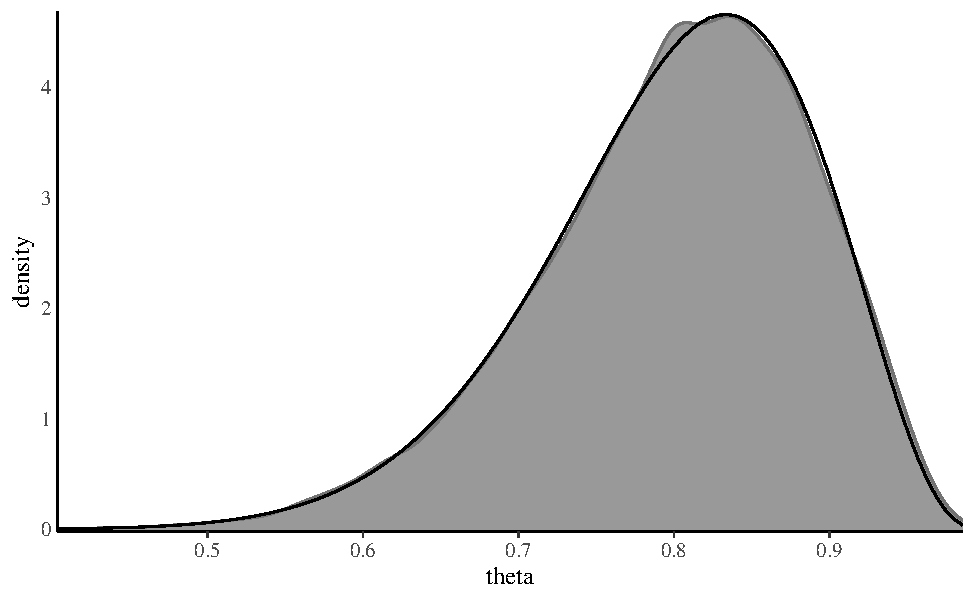
\includegraphics{ds4psy_files/figure-latex/hist-post-gautret-plus-correct-1} 

}

\caption{Istogramma che illustra l'approssimazione della distribuzione a posteriori per il parametro $\theta$ nel modello Beta-Binomiale. La curva nera rappresenta la corretta distribuzione a posteriori Beta(16, 4).}\label{fig:hist-post-gautret-plus-correct}
\end{figure}

Un intervallo di credibilità al 95\% per \(\theta\) si ottiene con la seguente chiamata:

\begin{Shaded}
\begin{Highlighting}[]
\NormalTok{posterior1 }\OtherTok{\textless{}{-}} \FunctionTok{extract}\NormalTok{(stanfit1)}
\NormalTok{rstantools}\SpecialCharTok{::}\FunctionTok{posterior\_interval}\NormalTok{(}\FunctionTok{as.matrix}\NormalTok{(stanfit1), }\AttributeTok{prob =} \FloatTok{0.95}\NormalTok{)}
\CommentTok{\#\textgreater{}          2.5\%    97.5\%}
\CommentTok{\#\textgreater{} theta   0.599   0.9376}
\CommentTok{\#\textgreater{} lp\_\_  {-}12.582 {-}10.0086}
\end{Highlighting}
\end{Shaded}

Svolgendo un'analisi bayesiana simile a questa, \citet{Gautret_2020} hanno trovato che gli intervalli di credibilità del gruppo di controllo e del gruppo sperimentale non si sovrappongono. Questo fatto viene interpretato dicendo che il parametro \(\theta\) è diverso nei due gruppi. Sulla base di queste evidenza, \citet{Gautret_2020} hanno concluso, con un grado di certezza soggettiva del 95\%, che nel gruppo sperimentale vi è una probabilità più bassa di risultare positivi al SARS-CoV-2 rispetto al gruppo di controllo. In altri termini, questa analisi dei dati suggerisce che l'idrossiclorochina sia efficace come terapia per il Covid-19.

\hypertarget{la-critica-di-hulme_2020}{%
\section{\texorpdfstring{La critica di \citet{Hulme_2020}}{La critica di @Hulme\_2020}}\label{la-critica-di-hulme_2020}}

Un articolo pubblicato da \citet{Hulme_2020} si è posto il problema di rianalizzare i dati di \citet{Gautret_2020}.\footnote{Si veda \url{https://osf.io/5dgmx/}.} Tra gli autori di questo articolo figura anche Eric-Jan Wagenmakers, uno psicologo molto conosciuto per i suoi contributi metodologici. \citet{Hulme_2020} hanno osservato che, nelle analisi statistiche riportate, \citet{Gautret_2020} hanno escluso alcuni dati. Nel gruppo sperimentale, infatti, vi erano alcuni pazienti i quali, anziché migliorare, sono in realtà peggiorati. L'analisi statistica di \citet{Gautret_2020} ha escluso i dati di questi pazienti. Se consideriamo tutti i pazienti --- non solo quelli selezionati da \citet{Gautret_2020} --- la situazione diventa la seguente:

\begin{itemize}
\tightlist
\item
  gruppo sperimentale: 10 positivi su 18;
\item
  gruppo di controllo: 14 positivi su 16.
\end{itemize}

L'analisi dei dati proposta da \citet{Hulme_2020} richiede l'uso di alcuni strumenti statistici che, in queste dispense, non verranno discussi. Ma possiamo giungere alle stesse conclusioni raggiunte da questi ricercatori anche usando le procedure statistiche descritte nel Paragrafo successivo.

\hypertarget{due-proporzioni}{%
\section{Due proporzioni}\label{due-proporzioni}}

Svolgiamo ora l'analisi considerando tutti i dati, come suggerito da \citet{Hulme_2020}. Per fare questo verrà creato un modello bayesiano per fare inferenza sulla differenza tra due proporzioni. Una volta generate le distribuzioni a posteriori per le proporzioni di ``successi'' nei due gruppi, verrà anche generata la quantità

\[
\omega = \frac{\theta_2 / (1-\theta_2)}{\theta_1 / (1-\theta_1)},
\]

ovvero il rapporto tra gli Odds di positività tra i pazienti del gruppo di controllo e gli Odds di positività tra i pazienti del gruppo sperimentale. Se il valore dell'OR è uguale a 1, significa che l'Odds di positività nel gruppo di controllo è uguale all'odds di positività nel gruppo sperimentale, cioè il fattore in esame (somministrazione dell'idrossiclorochina) è ininfluente sulla comparsa della malattia. L'inferenza statistica sull'efficacia dell'idrossiclorochina come terapia per il Covid-19 può dunque essere effettuata esaminando l'intervallo di credibilità al 95\% per l'OR: se tale intervallo include il valore 1, allora non vi è evidenza che l'idrossiclorochina sia efficace come terapia per il Covid-19.

Nell'implementazione di questo modello, la quantità di interesse è dunque l'odds ratio; tale quantità viene calcolata nel blocco \texttt{generated\ quantities} del programma Stan. In questo esempio useremo delle distribuzioni a priori vagamente informative per i parametri \(\theta_1\) e \(\theta_1\).

\begin{Shaded}
\begin{Highlighting}[]
\NormalTok{data\_list }\OtherTok{\textless{}{-}} \FunctionTok{list}\NormalTok{(}
  \AttributeTok{N1 =} \DecValTok{18}\NormalTok{, }
  \AttributeTok{y1 =} \DecValTok{10}\NormalTok{, }
  \AttributeTok{N2 =} \DecValTok{16}\NormalTok{, }
  \AttributeTok{y2 =} \DecValTok{14}
\NormalTok{)}
\end{Highlighting}
\end{Shaded}

\begin{Shaded}
\begin{Highlighting}[]
\NormalTok{modelString }\OtherTok{=} \StringTok{"}
\StringTok{//  Comparison of two groups with Binomial}
\StringTok{data \{}
\StringTok{  int\textless{}lower=0\textgreater{} N1;              // number of experiments in group 1}
\StringTok{  int\textless{}lower=0\textgreater{} y1;              // number of deaths in group 1}
\StringTok{  int\textless{}lower=0\textgreater{} N2;              // number of experiments in group 2}
\StringTok{  int\textless{}lower=0\textgreater{} y2;              // number of deaths in group 2}
\StringTok{\}}
\StringTok{parameters \{}
\StringTok{  real\textless{}lower=0,upper=1\textgreater{} theta1; // probability of death in group 1}
\StringTok{  real\textless{}lower=0,upper=1\textgreater{} theta2; // probability of death in group 2}
\StringTok{\}}
\StringTok{model \{}
\StringTok{  theta1 \textasciitilde{} beta(2, 2);          // prior}
\StringTok{  theta2 \textasciitilde{} beta(2, 2);          // prior}
\StringTok{  y1 \textasciitilde{} binomial(N1, theta1);    // observation model / likelihood}
\StringTok{  y2 \textasciitilde{} binomial(N2, theta2);    // observation model / likelihood}
\StringTok{\}}
\StringTok{generated quantities \{}
\StringTok{  // generated quantities are computed after sampling}
\StringTok{  real oddsratio = (theta2/(1{-}theta2))/(theta1/(1{-}theta1));}
\StringTok{\}}
\StringTok{"}
\FunctionTok{writeLines}\NormalTok{(modelString, }\AttributeTok{con =} \StringTok{"code/twoprop1.stan"}\NormalTok{)}
\end{Highlighting}
\end{Shaded}

\begin{Shaded}
\begin{Highlighting}[]
\NormalTok{file }\OtherTok{\textless{}{-}} \FunctionTok{file.path}\NormalTok{(}\StringTok{"code"}\NormalTok{, }\StringTok{"twoprop1.stan"}\NormalTok{)}
\end{Highlighting}
\end{Shaded}

\begin{Shaded}
\begin{Highlighting}[]
\NormalTok{mod }\OtherTok{\textless{}{-}} \FunctionTok{cmdstan\_model}\NormalTok{(file)}
\end{Highlighting}
\end{Shaded}

\begin{Shaded}
\begin{Highlighting}[]
\NormalTok{fit }\OtherTok{\textless{}{-}}\NormalTok{ mod}\SpecialCharTok{$}\FunctionTok{sample}\NormalTok{(}
  \AttributeTok{data =}\NormalTok{ data\_list,}
  \AttributeTok{iter\_sampling =}\NormalTok{ 4000L,}
  \AttributeTok{iter\_warmup =}\NormalTok{ 2000L,}
  \AttributeTok{seed =}\NormalTok{ SEED,}
  \AttributeTok{chains =}\NormalTok{ 4L,}
  \AttributeTok{parallel\_chains =}\NormalTok{ 4L,}
  \AttributeTok{refresh =} \DecValTok{0}\NormalTok{,}
  \AttributeTok{thin =} \DecValTok{1}
\NormalTok{)}
\end{Highlighting}
\end{Shaded}

\begin{Shaded}
\begin{Highlighting}[]
\NormalTok{stanfit }\OtherTok{\textless{}{-}}\NormalTok{ rstan}\SpecialCharTok{::}\FunctionTok{read\_stan\_csv}\NormalTok{(fit}\SpecialCharTok{$}\FunctionTok{output\_files}\NormalTok{())}
\end{Highlighting}
\end{Shaded}

\begin{Shaded}
\begin{Highlighting}[]
\FunctionTok{print}\NormalTok{(}
\NormalTok{  stanfit,}
  \AttributeTok{pars =} \FunctionTok{c}\NormalTok{(}\StringTok{"theta1"}\NormalTok{, }\StringTok{"theta2"}\NormalTok{, }\StringTok{"oddsratio"}\NormalTok{),}
  \AttributeTok{digits\_summary =}\NormalTok{ 3L}
\NormalTok{)}
\CommentTok{\#\textgreater{} Inference for Stan model: twoprop1{-}202201270929{-}1{-}5c8c8b.}
\CommentTok{\#\textgreater{} 4 chains, each with iter=6000; warmup=2000; thin=1; }
\CommentTok{\#\textgreater{} post{-}warmup draws per chain=4000, total post{-}warmup draws=16000.}
\CommentTok{\#\textgreater{} }
\CommentTok{\#\textgreater{}            mean se\_mean    sd  2.5\%   25\%   50\%   75\%}
\CommentTok{\#\textgreater{} theta1    0.546   0.001 0.103 0.344 0.475 0.546 0.620}
\CommentTok{\#\textgreater{} theta2    0.798   0.001 0.087 0.601 0.744 0.808 0.862}
\CommentTok{\#\textgreater{} oddsratio 4.721   0.043 4.411 0.906 2.166 3.514 5.698}
\CommentTok{\#\textgreater{}            97.5\% n\_eff Rhat}
\CommentTok{\#\textgreater{} theta1     0.740 12795    1}
\CommentTok{\#\textgreater{} theta2     0.937 14193    1}
\CommentTok{\#\textgreater{} oddsratio 15.558 10400    1}
\CommentTok{\#\textgreater{} }
\CommentTok{\#\textgreater{} Samples were drawn using NUTS(diag\_e) at Gio Gen 27 09:29:15 2022.}
\CommentTok{\#\textgreater{} For each parameter, n\_eff is a crude measure of effective sample size,}
\CommentTok{\#\textgreater{} and Rhat is the potential scale reduction factor on split chains (at }
\CommentTok{\#\textgreater{} convergence, Rhat=1).}
\end{Highlighting}
\end{Shaded}

L'intervallo di credibilità del 95\% per l'OR include il valore di 1.0 (ovvero, il valore che indica che gli odds di positività sono uguali nei due gruppi). In base agli standard correnti, un risultato di questo tipo non viene considerato come evidenza sufficiente per potere concludere che il parametro \(\theta\) assume un valore diverso nei due gruppi. In altri termini, se consideriamo tutti i dati, e non solo quelli selezionati dagli autori della ricerca originaria, non vi è evidenza alcuna che l'idrossiclorochina sia efficace come terapia per il Covid-19.

\hypertarget{commenti-e-considerazioni-finali-1}{%
\section*{Commenti e considerazioni finali}\label{commenti-e-considerazioni-finali-1}}


Concludiamo questa discussione dicendo che ciò che è stato presentato in questo capitolo è un esercizio didattico: la ricerca di \citet{Gautret_2020} include tante altre informazioni che non sono state qui considerate. Tuttavia, notiamo che la semplice analisi statistica che abbiamo qui descritto è stata in grado di replicare le conclusioni a cui sono giunti (per altra via) \citet{Hulme_2020}.

\mainmatter

\hypertarget{part-appendici}{%
\part{Appendici}\label{part-appendici}}

\hypertarget{appendix-appendici}{%
\appendix \addcontentsline{toc}{chapter}{\appendixname}}


\hypertarget{appendix:intro-stan}{%
\chapter{Programmare in Stan}\label{appendix:intro-stan}}

\hypertarget{interfacce-e-pacchetti}{%
\section{Interfacce e pacchetti}\label{interfacce-e-pacchetti}}

È possibile accedere al linguaggio Stan tramite diverse interfacce:

\begin{itemize}
\tightlist
\item
  \texttt{CmdStan}: eseguibile da riga di comando,
\item
  \texttt{RStan} - integrazione con il linguaggio \(\R\);
\item
  \texttt{PyStan} - integrazione con il linguaggio di programmazione Python;
\item
  \texttt{MatlabStan} - integrazione con MATLAB;
\item
  \texttt{Stan.jl} - integrazione con il linguaggio di programmazione Julia;
\item
  \texttt{StataStan} - integrazione con Stata.
\end{itemize}

Inoltre, vengono fornite interfacce di livello superiore con i pacchetti che utilizzano Stan come backend, principalmente in Linguaggio \R:

\begin{itemize}
\tightlist
\item
  \texttt{shinystan}: interfaccia grafica interattiva per l'analisi della distribuzione a posteriori e le diagnostiche MCMC;
\item
  \texttt{bayesplot}: insieme di funzioni utilizzabili per creare grafici relativi all'analisi della distribuzione a posteriori, ai test del modello e alle diagnostiche MCMC;
\item
  \texttt{brms}: fornisce un'ampia gamma di modelli lineari e non lineari specificando i modelli statistici mediante la sintassi usata in \R;
\item
  \texttt{rstanarm}: fornisce un sostituto per i modelli frequentisti forniti da base \(\R\) e \texttt{lme4} utilizzando la sintassi usata in \(\R\) per la specificazione dei modelli statistici;
\item
  \texttt{edstan}: modelli Stan per la Item Response Theory;
\item
  \texttt{cmdstanr}, un'interfaccia \(\R\) per \texttt{CmdStan}.
\end{itemize}

\hypertarget{interfaccia-cmdstanr}{%
\section{\texorpdfstring{Interfaccia \texttt{cmdstanr}}{Interfaccia cmdstanr}}\label{interfaccia-cmdstanr}}

Negli esempi di questa dispensa verrà usata l'interfaccia \texttt{cmdstanr}. Il pacchetto \texttt{cmdstanr} non è ancora disponibile su CRAN, ma può essere installato come indicato su questo \href{https://mc-stan.org/docs/2_27/cmdstan-guide/cmdstan-installation.html}{link}. Una volta che è stato installato, il pacchetto \texttt{cmdstanr} può essere caricato come un qualsiasi altro pacchetto R.

Si noti che \texttt{cmdstanr} richiede un'installazione funzionante di \texttt{CmdStan}, l'interfaccia shell per Stan. Se \texttt{CmdStan} non è installato, \texttt{cmdstanr} lo installerà automaticamente se il computer dispone di una \emph{Toolchain} adatta. Stan richiede infatti che sul computer su cui viene installato siano presenti alcuni strumenti necessari per gestire i file C++. Tra le altre ragioni, questo è dovuto al fatto che il codice Stan viene tradotto in codice C++ e compilato. Il modo migliore per ottenere il software necessario per un computer Windows o Mac è quello di installare \texttt{RTools}. Per un computer Linux, è necessario installare \texttt{build-essential} e una versione recente dei compilatori g++ o clang++. I requisiti sono descritti nella \href{https://mc-stan.org/docs/cmdstan-guide/cmdstan-installation.html}{Guida di CmdStan}.

Per verificare che la Toolchain sia configurata correttamente è possibile utilizzare la funzione \texttt{check\_cmdstan\_toolchain()}:

\begin{Shaded}
\begin{Highlighting}[]
\FunctionTok{check\_cmdstan\_toolchain}\NormalTok{()}
\end{Highlighting}
\end{Shaded}

Se la toolchain è configurata correttamente, \texttt{CmdStan} può essere installato mediante la funzione \texttt{install\_cmdstan()}:

\begin{Shaded}
\begin{Highlighting}[]
\CommentTok{\# do not run!}
\CommentTok{\# install\_cmdstan(cores = 2)}
\end{Highlighting}
\end{Shaded}

La versione installata di \texttt{CmdStan} si ottiene con:

\begin{Shaded}
\begin{Highlighting}[]
\FunctionTok{cmdstan\_version}\NormalTok{()}
\CommentTok{\#\textgreater{} [1] "2.28.2"}
\end{Highlighting}
\end{Shaded}

\hypertarget{codice-stan}{%
\section{Codice Stan}\label{codice-stan}}

Qualunque sia l'interfaccia che viene usata, i modelli sottostanti sono sempre scritti nel linguaggio Stan, il che significa che lo stesso codice Stan è valido per tutte le interfacce possibili. Il codice Stan è costituito da una serie di blocchi che vengono usati per specificare un modello statistico. In ordine, questi blocchi sono: \texttt{data}, \texttt{transformed\ data}, \texttt{parameters}, \texttt{transformed\ parameters}, \texttt{model}, e \texttt{generated\ quantities}.

\hypertarget{hello-world-stan}{%
\subsection{``Hello, world'' -- Stan}\label{hello-world-stan}}

Quando si studia un nuovo linguaggio di programmazione si utilizza spesso un programma ``Hello, world''. Questo è un modo semplice, spesso minimo, per dimostrare alcune delle sintassi di base del linguaggio. In Python, il programme ``Hello, world'' program è:

\begin{Shaded}
\begin{Highlighting}[]
\BuiltInTok{print}\NormalTok{(}\StringTok{"Hello, world."}\NormalTok{)}
\end{Highlighting}
\end{Shaded}

Qui presentiamo Stan e scriviamo un programma ``Hello, world'' per Stan.

Prima di scrivere il nostro primo programma ``Hello, world'' per Stan (che estrarrà campioni dalla distribuzione a posteriori di un modello gaussiano) spendiamo due parole per spiegare cosa fa Stan. Un utente scrive un modello usando il linguaggio Stan. Questo è solitamente memorizzato in un file di testo \texttt{.stan}. Il modello viene compilato in due passaggi. Innanzitutto, Stan traduce il modello nel file \texttt{.stan} in codice C++. Quindi, quel codice C++ viene compilato in codice macchina. Una volta creato il codice macchina, l'utente può, tramite l'interfaccia CmdStan, campionare la distribuzione definita dal modello ed eseguire altri calcoli con il modello. I risultati del campionamento vengono scritti su disco come file CSV e txt. Come mostrato di seguito, l'utente accede a questi file utilizzando varie funzioni \(\R\), senza interagire direttamente con loro.

Per iniziare, possiamo dire che un programma Stan contiene tre ``blocchi'' obbligatori: blocco \texttt{data}, blocco \texttt{parameters}, blocco \texttt{model}.

\hypertarget{blocco-data}{%
\subsection{\texorpdfstring{Blocco \texttt{data}}{Blocco data}}\label{blocco-data}}

Qui vengono dichiarate le variabili che saranno passate a Stan. Devono essere elencati i nomi delle variabili che saranno utilizzate nel programma, il \emph{tipo di dati} da registrare per ciascuna variabile, per esempio:

\begin{itemize}
\tightlist
\item
  \emph{int} = intero,
\item
  \emph{real} = numeri reali (ovvero, numeri con cifre decimali),
\item
  \emph{vector} = sequenze ordinate di numeri reali unidimensionali,
\item
  \emph{matrix} = matrici bidimensionali di numeri reali,
\item
  \emph{array} = sequenze ordinate di dati multidimensionali.
\end{itemize}

Devono anche essere dichiarate le dimensioni delle variabili e le eventuali restrizioni sulle variabili (es. \texttt{upper\ =\ 1} \texttt{lower\ =\ 0}, che fungono da controlli per Stan). Tutti i nomi delle variabili assegnate qui saranno anche usati negli altri blocchi del programma.

Per esempio, l'istruzione seguente dichiaria la variabile \texttt{Y} -- la quale rappresenta, ad esempio, l'altezza di 10 persone -- come una variabile di tipo \texttt{real{[}10{]}}. Ciò significa che specifichiamo un array di lunghezza 10, i cui elementi sono variabili continue definite sull'intervallo dei numeri reali \([-\infty, +\infty]\).

\begin{Shaded}
\begin{Highlighting}[]
\NormalTok{data \{}
\NormalTok{  real Y[}\DecValTok{10}\NormalTok{]; }\SpecialCharTok{/}\ErrorTok{/}\NormalTok{ heights }\ControlFlowTok{for} \DecValTok{10}\NormalTok{ people}
\NormalTok{\}}
\end{Highlighting}
\end{Shaded}

Invece, con l'istruzione

\begin{Shaded}
\begin{Highlighting}[]
\NormalTok{data \{}
\NormalTok{  int Y[}\DecValTok{10}\NormalTok{]; }\SpecialCharTok{/}\ErrorTok{/}\NormalTok{ qi }\ControlFlowTok{for} \DecValTok{10}\NormalTok{ people}
\NormalTok{\}}
\end{Highlighting}
\end{Shaded}

dichiariamo la variabile \texttt{Y} -- la quale rappresenta, ad esempio, il QI di 10 persone -- come una variabile di tipo \texttt{int{[}10{]}}, ovvero un array di lunghezza 10, i cui elementi sono numeri naturali, cioè numeri interi non negativi \(\{0, +1, +2, +3, +4, \dots\}\).

Un altro esempio è

\begin{Shaded}
\begin{Highlighting}[]
\NormalTok{data \{}
\NormalTok{  real}\SpecialCharTok{\textless{}}\NormalTok{lower}\OtherTok{=}\DecValTok{0}\NormalTok{, upper}\OtherTok{=}\DecValTok{1}\SpecialCharTok{\textgreater{}}\NormalTok{ Y[}\DecValTok{10}\NormalTok{]; }\SpecialCharTok{/}\ErrorTok{/} \DecValTok{10}\NormalTok{ proportions}
\NormalTok{\}}
\end{Highlighting}
\end{Shaded}

nel quale viene specificato un array di lunghezza 10, i cui elementi sono delle variabili continue definite sull'intervallo dei numeri reali \([0, 1]\) --- per esempio, delle proporzioni.

Si noti che i tipi \texttt{vector} e \texttt{matrix} contengono solo elementi di tipo \texttt{real}, ovvero variabili continue, mentre gli \texttt{array} possono contenere dati di qualsiasi tipo. I dati passati a Stan devono essere contenuti in un oggetto del tipo \texttt{list}.

\hypertarget{blocco-parameters}{%
\subsection{\texorpdfstring{Blocco \texttt{parameters}}{Blocco parameters}}\label{blocco-parameters}}

I parametri che vengono stimati sono dichiarati nel blocco \texttt{parameters}. Per esempio, l'istruzione

\begin{Shaded}
\begin{Highlighting}[]
\NormalTok{parameters \{}
\NormalTok{  real mu; }\SpecialCharTok{/}\ErrorTok{/}\NormalTok{ mean height }\ControlFlowTok{in}\NormalTok{ population}
\NormalTok{  real}\SpecialCharTok{\textless{}}\NormalTok{lower}\OtherTok{=}\DecValTok{0}\SpecialCharTok{\textgreater{}}\NormalTok{ sigma; }\SpecialCharTok{/}\ErrorTok{/}\NormalTok{ sd of height distribution}
\NormalTok{\}}
\end{Highlighting}
\end{Shaded}

dichiaria la variabile \texttt{mu} che codifica l'altezza media nella popolazione, che è una variabile continua in un intervallo illimitato di valori, e la deviazione standard \texttt{sigma}, che è una variabile continua non negativa. Avremmo anche potuto specificare un limite inferiore di zero su \texttt{mu} perché deve essere non negativo.

Per una regressione lineare semplice, ad esempio, devono essere dichiarate le variabili corrispondenti all'intercetta (\texttt{alpha}), alla pendenza (\texttt{beta}) e alla deviazione standard degli errori attorno alla linea di regressione (\texttt{sigma}). In altri termini, nel blocco \texttt{parameters} devono essere elencati tutti i parametri che dovranno essere stimati dal modello. Si noti che parametri discreti non sono possibili. Infatti, Stan attualmente non supporta i parametri con valori interi, almeno non direttamente.

\hypertarget{blocco-model}{%
\subsection{\texorpdfstring{Blocco \texttt{model}}{Blocco model}}\label{blocco-model}}

Nel blocco \texttt{model} vengono elencate le dichiarazioni relative alla verosimiglianza dei dati e alle distribuzioni a priori dei parametri, come ad esempio, nelle istruzioni seguenti.

\begin{Shaded}
\begin{Highlighting}[]
\NormalTok{model \{}
  \ControlFlowTok{for}\NormalTok{(i }\ControlFlowTok{in} \DecValTok{1}\SpecialCharTok{:}\DecValTok{10}\NormalTok{) \{}
\NormalTok{    Y[i] }\SpecialCharTok{\textasciitilde{}} \FunctionTok{normal}\NormalTok{(mu, sigma);}
\NormalTok{  \}}
\NormalTok{  mu }\SpecialCharTok{\textasciitilde{}} \FunctionTok{normal}\NormalTok{(}\DecValTok{170}\NormalTok{, }\DecValTok{15}\NormalTok{); }\SpecialCharTok{/}\ErrorTok{/}\NormalTok{ prior }\ControlFlowTok{for}\NormalTok{ mu}
\NormalTok{  sigma }\SpecialCharTok{\textasciitilde{}} \FunctionTok{cauchy}\NormalTok{(}\DecValTok{0}\NormalTok{, }\DecValTok{20}\NormalTok{); }\SpecialCharTok{/}\ErrorTok{/}\NormalTok{ prior }\ControlFlowTok{for}\NormalTok{ sigma}
\NormalTok{\}}
\end{Highlighting}
\end{Shaded}

Mediante l'istruzione all'interno del ciclo \texttt{for}, ciascun valore dell'altezza viene concepito come una variable casuale proveniente da una distribuzione Normale di parametri \(\mu\) e \(\sigma\) (i parametri di interesse nell'inferenza). Il ciclo \texttt{for} viene ripetuto 10 volte perché i dati sono costituiti da un array di 10 elementi (ovvero, il campione è costituito da 10 osservazioni).

Le due righe che seguno il ciclo \texttt{for} specificano le distribuzioni a priori dei parametri su cui vogliamo effettuare l'inferenza. Per \(\mu\) assumiamo una distribuzione a priori Normale di parametri \(\mu = 170\) e \(\sigma = 15\); per \(\sigma\) assumiamo una distribuzione a priori Cauchy(0, 20).

Se non viene definita alcuna distribuzione a priori, Stan utilizzerà la distribuzione a priori predefinita \(Unif(-\infty, +\infty)\). Raccomandazioni sulle distribuzioni a priori sono fornite in questo \href{https://github.com/stan-dev/stan/wiki/Prior-Choice-Recommendations}{link}.

La precedente notazione di campionamento può anche essere espressa usando la seguente notazione alternativa:

\begin{Shaded}
\begin{Highlighting}[]
  \ControlFlowTok{for}\NormalTok{(i }\ControlFlowTok{in} \DecValTok{1}\SpecialCharTok{:}\DecValTok{10}\NormalTok{) \{}
\NormalTok{    target }\SpecialCharTok{+}\ErrorTok{=} \FunctionTok{normal\_lpdf}\NormalTok{(Y[i] }\SpecialCharTok{|}\NormalTok{ mu, sigma);}
\NormalTok{  \}}
\end{Highlighting}
\end{Shaded}

Questa notazione rende trasparente il fatto che, in pratica, Stan esegue un campionamento nello spazio

\[
\log p(\theta \mid y) \propto \log p(y \mid \theta) + \log p(\theta) = \sum_{i=1}^n \log p(y_i \mid \theta) + \log p(\theta).
\]

Per ogni passo MCMC, viene ottenuto un nuovo valore di \(\mu\) e \(\sigma\) eviene valutata la log densità a posteriori non normalizzata. Ad ogni passo MCMC, Stan calcola un nuovo valore della densità a posteriori su scala logaritmica partendo da un valore di 0 e incrementandola ogni volta che incontra un'istruzione \texttt{\textasciitilde{}}. Quindi, le istruzioni precedenti aumentano la log-densità di una quantità pari a \(\log (p(Y[i])) \propto -\frac{1}{2} \log(\sigma^2) - (Y[i]-\mu)^2 / 2\sigma^2\) per le altezze si ciascuno degli \(i=1 \dots, 10\) individui -- laddove la formula esprime, in termini logaritmici, la densità Normale da cui sono stati esclusi i termini costanti.

Oppure, in termini vettorializzati, il modello descritto sopra può essere espresso come

\begin{Shaded}
\begin{Highlighting}[]
\NormalTok{model \{}
\NormalTok{  Y }\SpecialCharTok{\textasciitilde{}} \FunctionTok{normal}\NormalTok{(mu, sigma);}
\NormalTok{\}}
\end{Highlighting}
\end{Shaded}

dove il termine a sinistra di \(\sim\) è un array. Questa notazione più compatta è anche la più efficiente.

\hypertarget{blocchi-opzionali}{%
\subsection{Blocchi opzionali}\label{blocchi-opzionali}}

Ci sono inoltre tre blocchi opzionali:

\begin{itemize}
\tightlist
\item
  Il blocco \texttt{transformed\ data} consente il pre-processing dei dati. È possibile trasformare i parametri del modello; solitamente ciò viene fatto nel caso dei modelli più avanzati per consentire un campionamento MCMC più efficiente.
\item
  Il blocco \texttt{transformed\ parameters} consente la manipolazione dei parametri prima del calcolo della distribuzione a posteriori.
\item
  Il blocco \texttt{generated\ quantities} consente il post-processing riguardante qualsiasi quantità che non fa parte del modello ma può essere calcolata a partire dai parametri del modello, per ogni iterazione dell'algoritmo. Esempi includono la generazione dei campioni a posteriori e le dimensioni degli effetti.
\end{itemize}

\hypertarget{sintassi}{%
\subsection{Sintassi}\label{sintassi}}

Si noti che il codice Stan richiede i punti e virgola (;) alla fine di ogni istruzione di assegnazione. Questo accade per le dichiarazioni dei dati, per le dichiarazioni dei parametri e ovunque si acceda ad un elemento di un tipo \texttt{data} e lo si assegni a qualcos'altro. I punti e virgola non sono invece richiesti all'inizio di un ciclo o di un'istruzione condizionale, dove non viene assegnato nulla.

In STAN, qualsiasi stringa che segue \texttt{//} denota un commento e viene ignorata dal programma.

Stan è un linguaggio estremamente potente e consente di implementare quasi tutti i modelli statistici, ma al prezzo di un certo sforzo di programmazione. Anche l'adattamento di semplici modelli statistici mediante il linguaggio STAN a volte può essere laborioso. Per molti modelli comunemente usati, come i modelli di regressione e multilivello, tale processo può essere semplificato usando le funzioni del pacchetto \texttt{brms}. D'altra parte, per modelli veramente complessi, non ci sono molte alternative all'uso di STAN. Per chi è curioso, il manuale del linguaggio Stan è accessibile al seguente \href{https://mc-stan.org/docs/2_27/stan-users-guide/index.html}{link}.

\hypertarget{workflow}{%
\section{Workflow}\label{workflow}}

Se usiamo \texttt{cmdstanr}, dobbiamo prima scrivere il codice con il modello statistico in un file in formato Stan. È necessario poi ``transpile'' quel file, ovvero tradurre il file in C++ e compilarlo. Ciò viene fatto mediante la funzione \texttt{cmdstan\_model()}. Possiamo poi eseguire il campionamento MCMC con il metodo \texttt{\$sample()}. Infine è possibile creare un sommario dei risultati usando, per esempio, usando il metodo \texttt{\$summary()}.

\hypertarget{ciao-stan}{%
\section{Ciao, Stan}\label{ciao-stan}}

Scriviamo ora il nostro programma Stan ``Hello, world'' per generare campioni da una distribuzione Normale standard (con media zero e varianza unitaria).

\begin{Shaded}
\begin{Highlighting}[]
\NormalTok{modelString }\OtherTok{=} \StringTok{"}
\StringTok{parameters \{}
\StringTok{  real x;}
\StringTok{\}}
\StringTok{model \{}
\StringTok{  x \textasciitilde{} normal(0, 1);}
\StringTok{\}}
\StringTok{"}
\FunctionTok{writeLines}\NormalTok{(modelString, }\AttributeTok{con =} \StringTok{"code/hello\_world.stan"}\NormalTok{)}
\end{Highlighting}
\end{Shaded}

Si noti che ci sono solo due blocchi in questo particolare codice Stan, il blocco parametri e il blocco modello. Questi sono due dei sette blocchi possibili in un codice Stan. Nel blocco parametri, abbiamo i nomi e i tipi di parametri per i quali vogliamo ottenere i campioni. In questo caso, vogliamo ottenere campioni di numeri reale che chiamiamo \texttt{x}. Nel blocco modello, abbiamo il nostro modello statistico. Specifichiamo che x, il parametro di cui vogliamo ottenere i campioni, è normalmente distribuito con media zero e deviazione standard unitaria. Ora che abbiamo il nostro codice (che è stato memorizzato in un file chiamato \texttt{hello\_world.stan}), possiamo usare CmdStan per compilarlo e ottenere \texttt{mod}, che è un oggetto \(\R\) che fornisce l'accesso all'eseguibile Stan compilato.

Leggiamo il file in cui abbiamo salvato il codice Stan

\begin{Shaded}
\begin{Highlighting}[]
\NormalTok{file }\OtherTok{\textless{}{-}} \FunctionTok{file.path}\NormalTok{(}\StringTok{"code"}\NormalTok{, }\StringTok{"hello\_world.stan"}\NormalTok{)}
\end{Highlighting}
\end{Shaded}

compiliamo il modello

\begin{Shaded}
\begin{Highlighting}[]
\NormalTok{mod }\OtherTok{\textless{}{-}} \FunctionTok{cmdstan\_model}\NormalTok{(file)}
\end{Highlighting}
\end{Shaded}

ed eseguiamo il campionamento MCMC:

\begin{Shaded}
\begin{Highlighting}[]
\NormalTok{fit }\OtherTok{\textless{}{-}}\NormalTok{ mod}\SpecialCharTok{$}\FunctionTok{sample}\NormalTok{(}
  \AttributeTok{iter\_sampling =}\NormalTok{ 4000L,}
  \AttributeTok{iter\_warmup =}\NormalTok{ 2000L,}
  \AttributeTok{seed =}\NormalTok{ SEED,}
  \AttributeTok{chains =}\NormalTok{ 4L,}
  \AttributeTok{refresh =} \DecValTok{0}\NormalTok{,}
  \AttributeTok{thin =} \DecValTok{1}
\NormalTok{)}
\end{Highlighting}
\end{Shaded}

Tasformiamo l'oggetto \texttt{fit} nel formato \texttt{stanfit} per manipolarlo più facilmente:

\begin{Shaded}
\begin{Highlighting}[]
\NormalTok{stanfit }\OtherTok{\textless{}{-}}\NormalTok{ rstan}\SpecialCharTok{::}\FunctionTok{read\_stan\_csv}\NormalTok{(fit}\SpecialCharTok{$}\FunctionTok{output\_files}\NormalTok{())}
\end{Highlighting}
\end{Shaded}

Lo esaminiamo

\begin{Shaded}
\begin{Highlighting}[]
\FunctionTok{length}\NormalTok{(stanfit}\SpecialCharTok{@}\NormalTok{sim}\SpecialCharTok{$}\NormalTok{samples)}
\CommentTok{\#\textgreater{} [1] 4}
\end{Highlighting}
\end{Shaded}

Quello che abbiamo ottenuto sono 4 catene di 4000 osservazioni ciascuna, le quali contengono valori casuali estratti dalla gaussiana standardizzata:

\begin{Shaded}
\begin{Highlighting}[]
\FunctionTok{head}\NormalTok{(stanfit}\SpecialCharTok{@}\NormalTok{sim}\SpecialCharTok{$}\NormalTok{samples[[}\DecValTok{1}\NormalTok{]])}
\end{Highlighting}
\end{Shaded}

Verifichiamo

\begin{Shaded}
\begin{Highlighting}[]
\FunctionTok{hist}\NormalTok{(stanfit}\SpecialCharTok{@}\NormalTok{sim}\SpecialCharTok{$}\NormalTok{samples[[}\DecValTok{1}\NormalTok{]][, }\DecValTok{1}\NormalTok{])}
\end{Highlighting}
\end{Shaded}

\begin{center}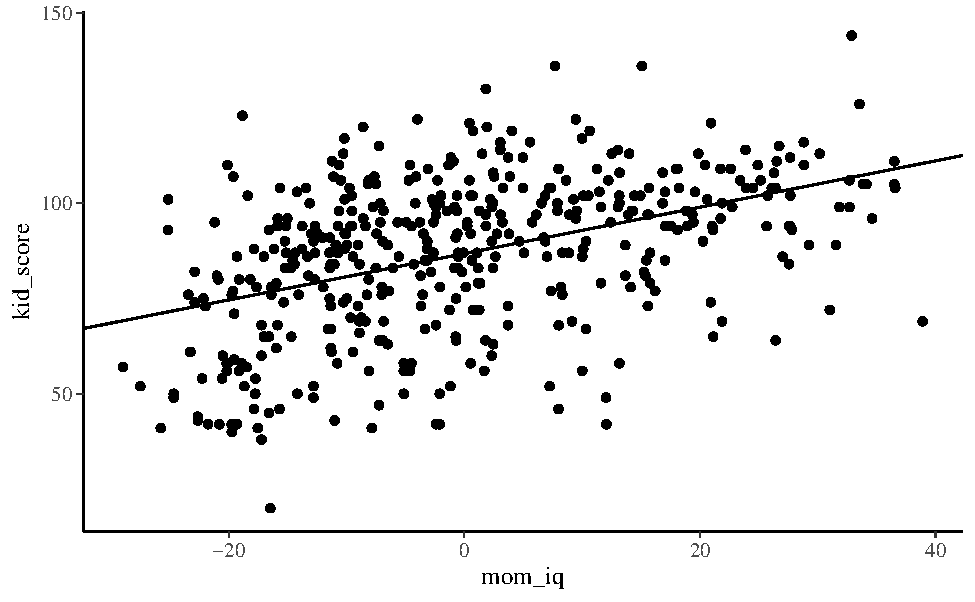
\includegraphics{ds4psy_files/figure-latex/unnamed-chunk-46-1} \end{center}

  \bibliography{refs.bib,book.bib,packages.bib}

\printindex

\end{document}
